%% LyX 2.2.2 created this file.  For more info, see http://www.lyx.org/.
%% Do not edit unless you really know what you are doing.
\documentclass[oneside,english]{amsbook}
\usepackage[T1]{fontenc}
\usepackage[utf8]{inputenc}
\usepackage{float}
\usepackage{amsbsy}
\usepackage{amstext}
\usepackage{amssymb}
\usepackage{graphicx}
\usepackage[authoryear]{natbib}

\makeatletter

%%%%%%%%%%%%%%%%%%%%%%%%%%%%%% LyX specific LaTeX commands.
%% Because html converters don't know tabularnewline
\providecommand{\tabularnewline}{\\}
\floatstyle{ruled}
\newfloat{algorithm}{tbp}{loa}
\providecommand{\algorithmname}{Algorithm}
\floatname{algorithm}{\protect\algorithmname}

%%%%%%%%%%%%%%%%%%%%%%%%%%%%%% Textclass specific LaTeX commands.
\numberwithin{section}{chapter}

%%%%%%%%%%%%%%%%%%%%%%%%%%%%%% User specified LaTeX commands.
\usepackage{amsmath}
\DeclareMathOperator*{\argmax}{arg\,max}
\DeclareMathOperator*{\argmin}{arg\,min}
\usepackage{dsfont}
\newcommand{\mathbbOld}{\mathbb}
\renewcommand{\mathbb}{\mathds}
\usepackage{natbib}
\usepackage{algorithm,algpseudocode}

\makeatother

\usepackage{babel}
\begin{document}
\tableofcontents{}\pagebreak{}

\chapter{Neural networks}

In this chapter, we will introduce concepts and techniques that are
used in artificial intelligence tasks. In particular, we will introduce
neural networks, that have proven a powerful model and produced state
of the art results in a variety of tasks.

\section{Artificial intelligence}

Intelligence is a difficult concept to define. We will use the following
definition: the ability to make sensible decisions in a given situation,
possibly making use of a memory of past events that share similarities
with the current situation. The most intelligent individual agent
that we are aware of nowadays is certainly the human being, amongst
other animals. Human beings are constantly making decisions given
their perception of the world that is provided by their 5 senses,
using knowledge that they have studied or experienced in their life.
But there is no \textit{a priori} reason to think that intelligence
could not be present in other systems, and in particular artificial
intelligence is a scientific field that aims at implementing intelligence
in non-living machines.

How our society of humans can benefit from artificial intelligence
is still an open question, out of the scope of the present document.
Regardless, given the recent popularity of artificial intelligence
among public research laboratories and in the industry, and the recent
successes at solving complex tasks, we can say without taking risks
that artificial intelligence will continue to play a big role in shaping
the future of our society.

From a more practical perspective, implementing an artificial intelligent
machine requires designing a system that takes data that represent
the current situation, data that represents the memory of the machine,
and output a decision using this data.

To put things into context, we will now describe an example task.
We want to design a program that takes a picture of an animal and
a sound as input, and outputs whether it thinks the animal present
in the picture makes the provided sound. In a computer, a picture
is often encoded as a mathematical tensor of scalar values or pixels,
the sound as a timeseries of samples of the sound wave, and the final
decision can be a single scalar values, which will be close to 0 is
the animal is very unlikely to make the noise, or to 1 if the animal
is very likely to make the noise. The complex machinery inbetween
is the intelligent part.

Manually designing a program for such a task is an overwhelming task.
Even provided that the input image is quite a small image of $32\times32$
RGB pixels and the sound lasts $1s$ recorded at a sample rate of
20kHz we have a total of $32\times32\times3+20\,000=23\,072$ scalars.
If we restrict each of these numbers to have $256$ possible values,
it leaves us with $256^{23\,072}\approx10^{55\,000}$ possible combinations.
Even if we only keep the combinations that are plausible, there is
too many to create a naive program. Even with carefully engineered
feature extractors based on image and sound processing techniques,
the remaining work of is still challenging.

Instead, the most successful attempts at solving such tasks use a
procedure called \textbf{machine learning}: instead of manually defining
our program, we define a generic model, and we use a dataset of annotated
examples of picture, sound, and the corresponding answer, and we leave
to the computer the task of extracting information from the dataset
to tune the model so as to obtain the desired program.

\section{Machine learning}

\subsection{Parametric functions and learning}

Generally speaking, machine learning consists in finding an unknown
function $f$ from a family of functions $\mathcal{F}$, that will
solve a certain task. We typically restrict our search to a smaller
family of functions, which consists in parametrized functions $\mathcal{F}_{\theta}$.
We will denote by $f_{\theta}$ such a function, parametrized by a
vector of parameters $\theta$. Adapting the value of the parameters
will change the output of the function $f_{\theta}$. The challenges
of machine learning are to find a correct parametrization so that
our desired function can be approached by a member of $\mathcal{F}_{\theta}$,
and to learn the parameters of this target function.

To this end, we need a measure of the performance of a given function
at solving our task. We chose a loss function $l$, adapted to this
task. The better our function, the lower the value of $l$. The remaining
ingredient is a data generating distribution $p$ from which we sample
datapoints $x\sim p$ that are our examples. A measure of the performance
of a function $f_{\theta}$ for the given task is given by the risk:\label{cost-function}

\begin{eqnarray*}
\mathcal{R}\left(\theta,p\right) & = & \mathbb{E}_{x\sim p}\left[l\left(f_{\theta}\left(x\right)\right)\right]
\end{eqnarray*}

$\mathcal{R}$ is a scalar value. If this value is high, then $f_{\theta}$
is bad at solving the desired task. In the opposite, the best function
can be found by adjusting $\theta$ so as to reach the smallest value
of $\mathcal{R}$. The best value for the parameter vector $\theta^{*}$
is given by:

\begin{eqnarray*}
\theta^{*} & = & \text{argmin}_{\theta}\mathcal{R}\left(\theta,p\right)
\end{eqnarray*}

Finding this value $\theta^{*}$ is the task of learning from the
data.

We now present two common tasks and their corresponding loss functions.
We will restrict to the less general setting of \textit{supervised}
learning, where each data point is composed of an input $x$ and a
target $y$.

In\textbf{ regression}, the input vector $x$ is mapped to a numerical
value $y$. To assess the performance of $f_{\theta}$, we use the
loss function $l\left(f_{\theta}\left(x\right),y\right)=\left\Vert f_{\theta}\left(x\right)-y\right\Vert _{2}^{2}$,
called the quadratic error. It reaches its minimum $0$ when $f_{\theta}\left(x\right)=y$.
For example we can design a model that predicts the price of a real
estate, given some features such as the size of the house, the number
of bedrooms and whether it possesses a fireplace.

In supervised \textbf{classification}, we classify each data point
$x$ into a category $y$. A natural loss that comes up is the misclassification
indicator function $\mathbf{1}\left(f_{\theta}\left(x\right),y\right)=\left\{ 0\text{ if }f_{\theta}\left(x\right)=y\text{ or }1\text{ otherwise}\right\} $.
It counts the examples that are misclassified. This function present
the disadvantage of not being differentiable (it is not even continuous),
and we will see in future sections that differentiability is a valuable
property for machine learning. Instead, we usually make our function
$f_{\theta}$ output a vector of the number of categories, which represents
computed probabilites of being a member of each category (a scalar
between $0$ and $1$). We use the loss called \textit{cross entropy
$l\left(f_{\theta}\left(x\right),y\right)=-\log\left(\left(f_{\theta}\left(x\right)\right)_{y}\right)$}.
This will push the probability of the correct category toward $1$.
An example classification task is proposed by the ImageNet project
\citep{deng2009imagenet} where the task is to classify images to
detect what they represent such as an animal, or a car and so on.

\subsection{Empirical risk and bias-variance tradeoff\label{subsec:Empirical-risk-and}}

In practice, often, we do not have access to a data generating function
$p$, but instead we have a limited number of samples from it. This
dataset of examples gives us an estimate of the true risk, by replacing
the expectation with a finite sum, called the empirical risk $R$:

\begin{align}
\begin{array}{ccccc}
\mathcal{R}\left(\theta,p\right) & \approx & R\left(\theta,\mathcal{D}\right) & = & \frac{1}{n}\sum_{x\in\mathcal{D}}l\left(f_{\theta}\left(x\right)\right)\end{array}\label{eq:empirical-risk}
\end{align}

$n$ is the total number of examples in $\mathcal{D}$.

For random values of the parameters $\theta$, the empirical risk
and the true risk will have similar values. But this is not the case
when the parameters have been tuned so that the empirical risk is
minimum. In the extreme case, consider a model that has memorized
all examples of the training set by heart. In order to make a prediction
for a new example, this model will seek the closest example in $\mathcal{D}$,
in term of the euclidean distance, and output the exact same answer
than this closest example. This model is called a 1-nearest neighbour
regressor or classifier regarding the considered task. In this case
the empirical risk is $0$, but we have no guarantee that the model
generalizes on new examples.

A model with too much expressivity, or \textit{variance}, will be
able to learn all examples in the training set by heart without having
the ability to generalize on new examples, which is called \textit{overfitting}.
A model with not enough expressivity will not be able to perform well
even on the training set, which is called \textit{underfitting}. In
the meantime it will have a similar performance on the true data generating
distribution. We say that there is a \textit{bias} toward a family
of model. The bias-variance tradeoff consists in selecting a model
that has sufficient expressivity to have a good performance on the
train set, while not having too much expressivity so that it will
not overfit, and still have good performance on the true data generating
distribution.

\subsection{Regularization}

A way of combatting overfitting is to use regularization. It is a
way of constraining the values of the parameters of a function using
priors. For example L2 regularization penalizes the squared norm of
the parameter vector. It constrains all values to stay small.

Data augmentation is another mean of combatting overfitting. We can
use the knowledge that we have of our dataset to create new examples.
For example for a classification task of images, we know from our
experience of the world that rotating or translating an image will
not change its content. We can thus artificially augment our training
set by including rotated and translated versions of the same images.

\section{Neural networks}

Neural networks are a family of parametrized models. They have empirically
proven very powerful at solving complex tasks. Along with the availability
of easy to use frameworks to build neural networks and learn from
data, has developed new interests from industry to integrate artificial
intelligence inspired techniques in more and more products. The first
commercial successes date back to the 90s when AT\&T developed an
automated system to read handwritten digits on bank checks, using
convolutional neural networks \citep{lecun1998gradient}. Recent successes
include advances in machine translation, image and voice recognition,
close-to-realistic image generation. They have applications in online
services integrated in smartphones, but also enable the invention
of new automated systems that will benefit more traditional industries,
(energy, agriculture, arts, ..)

\section{Common types of neural networks}

\subsection{Multilayer perceptron}

We now define the simplest neural network structure called the perceptron
\citep{rosenblatt1961principles}. From an input data vector $x$,
it creates a prediction $y$ using the relation $y\left(x\right)=f\left(\left\langle w,x\right\rangle +b\right)$.
$w$ is called the weight vector, and $b$ is the bias. $f$ is a
function, and is sometimes called the nonlinearity or activation function
as it allows the function $y$ to be different than just a linear
function of its input $x$. From a trained perceptron, we take a decision
for an example $x$ by comparing the value of the corresponding $y$
using a threshold value. Perceptrons were implemented before the invention
of modern computers, as complex electronic circuits. The weights were
encoded in hardware potentiometers and trained using an error-propagating
process. Remarkably, these complex pieces of machinery were capable
of obtaining good results for the task of recognizing simple shape
images.

These perceptrons were designed to approximately replicate the computations
made by a network of biological neurons. Each neuron gets input data
from several other neurons, consisting in voltage spikes. The rate
at which these spikes occur can be intepreted as whether a neuron
is excited or not. Each neuron has different sensibilities regarding
how it will react to an increase in spike rate from other neurons,
this sensibility being mimicked by the weights in artificial neural
networks. In its most simple modeling, the human brain is just a very
complex network of these neurons. This is the inspiration for artificial
neural networks.

This single perceptron is extended in a more complex model called
the multilayer perceptron (MLP). It consists in alternatively stacking
layers of linear transformation $a=Wx+b$ and nonlinearities $y=f\left(a\right)$,
using a vectorized generalization of the perceptron: $y\left(x\right)=f\left(Wx+b\right)$.
$W$ is now a weight matrix, and $b$ a bias vector. $f$ is often
an elementwise function. We stack these transformations to get more
complex functions. An example for 2 layers gives a function $y\left(x\right)=f_{2}\left(W_{2}f_{1}\left(W_{1}x+b_{1}\right)+b_{2}\right)$.
The intermediate values obtained at each layer $f_{1}\left(W_{1}x+b_{1}\right)$
are called the hidden representations as they are new representations
of the same input data, but encoded in a different way. A trained
neural network will create representations that are better suited
for its task. For example, if we imagine a task of classifying images
between those which picture a dog and those with a cat, we are interested
in a high level representation of characteristics such as a long tail,
whiskers or sharp ears.

\begin{figure}
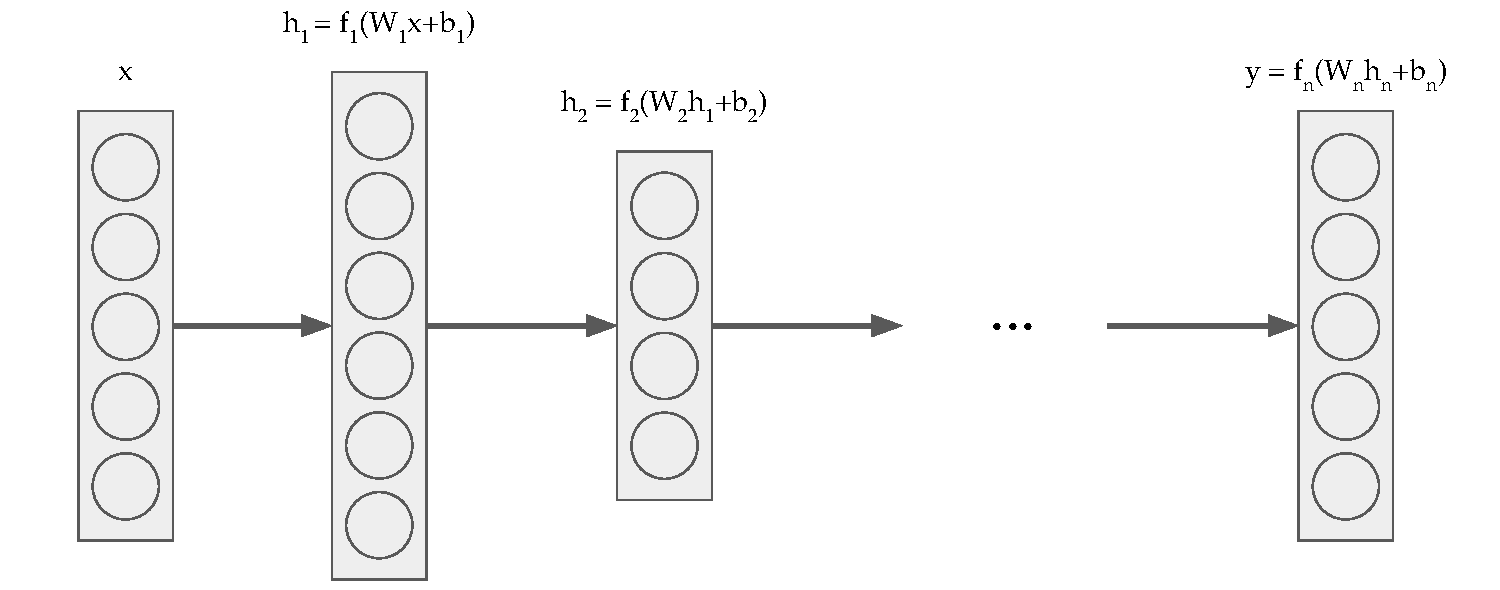
\includegraphics[width=1\textwidth]{figures/mlp}\caption{A multilayer perceptron consists in alternatively stacking layers
of a linear transformation and a nonlinearity}
\end{figure}


\subsection{Convolutional networks}

Convolutional networks \citep{lecun1989backpropagation} are well-suited
for tasks involving sequential (timeseries) or spatial data (images).
Instead of multiplying a weight matrix with the whole input vector
as in MLPs, we split this input into smaller chunks of fixed sized
corresponding to small vectors (1d case) or small matrices (2d case).
The same weight matrix is applied to each of this smaller vectors
so as to get a result at each position. In fact it amounts to a standard
MLP with sparse connectivity and with the weight matrix sharing values
between corresponding positions.

\subsection{Autoencoders\label{subsec:Autoencoders}}

Autoencoders \citep{hinton2006reducing,vincent2008extracting} are
neural networks that are composed of an encoder part a decoder. The
encoder takes the input and encodes encodes it to a new representation
(often with less dimension than the input). The decoder takes the
encoded input with the task of reconstructing the output. The encoded
representation is often a layer with less neurons than the size of
the input. The autoencoder is trained end-to-end, without manually
taking care of the encoded representation. This representation is
automatically created by learning from the data. It is a special case
for regression. In order to be efficient, a well designed autoencoder
will need to create a relevant representation of the data. For example,
if we want to encode pictures of faces, relevant representations could
be the gender, the color and size of hair, and so on.

\section{More elaborated cost functions}

We can often associate a task and its corresponding loss function:
regression with the quadratic error loss, and classification with
the cross entropy loss \ref{cost-function}. Some more recent advances
in neural networks make use of more complex cost functions.

\textbf{Neural art }\citep{gatys2015neural} and its feed-forward
extension \citep{ulyanov2016texture} tackle the task of generating
artwork images from a real world picture, that mimick the style of
a given painting. To this end, they create a cost function that measures
how a generated image resembles both the picture and the painting:

\begin{eqnarray*}
\mathcal{L}_{\text{total}}\left(p,a,x\right) & = & \alpha\mathcal{L}_{\text{content}}\left(p,x\right)+\beta\mathcal{L}_{\text{style}}\left(a,x\right)
\end{eqnarray*}

$p$ is the picture, $a$ is the artwork that we want to extract the
style, and $x$ is any image. $\mathcal{L}_{\text{content}}$ is a
loss function that measures how close $x$ is from $p$ in terms of
contents, and $\mathcal{L}_{\text{style}}$ is a loss function that
measures a distance from $a$ to $x$ in terms of artistic style.
By minimizing $\mathcal{L}_{\text{total}}\left(p,a,x\right)$ with
respect to $x$ for given $p$ and $a$, we obtain the desired image
in $x$. $\alpha$ and $\beta$ are scalar values that control the
influence of each part of the loss. In the original paper \citep{gatys2015neural}
we start from a randomly initialized $x$ and we perform gradient
descent on each pixel of $x$. In \citet{ulyanov2016texture} we use
a convolutional neural network to generate $x$, which takes the picture
as input, and outputs the desired stylized image. This network is
trained using $\mathcal{L}_{\text{total}}$. It has the main advantage
of being very fast as generating new images once it has be trained
on a specific artwork.

Another family of cost functions that becomes more and more popular
is that of the discriminators in \textbf{Generative Adversarial Networks
}\citep{goodfellow2014generative}, that can be thought of as learned
cost functions. In this setup, 2 networks are trained one against
each other : the generator part takes random noise and generate a
sample that tries to fool the discriminator. The discriminator also
is a trained network that tries to classify whether its input is from
a given data distribution, or if it was generated by the generator.
Training these networks is very unstable, and is the object of many
research at the time of this writing. But provided that we successfully
trained both parts, we get a generator that is able to generate new
samples of complex data, such as realistic images.

\chapter{Optimization of neural networks}

\section{Gradient descent and backpropagation\label{sec:Gradient-descent-and}}

\subsection{Learning using gradient descent}

Once we have chosen a model, and supposing that this model is capable
of solving a given task with a dataset of examples of this task, the
main challenge is now to learn the parameters of the model from the
data. Some simple models have closed form solutions, this is for example
the case for a linear model and a regression task. For more complex
models such as neural networks, we can not derive a simple formula
for getting the values of all parameters given a dataset. In this
case, we start from an initialized network and iterate updates for
our parameters until we get the expected results. To this end, we
must find an efficient way of getting an update $\Delta\theta$ of
our parameters $\theta$. Considering that we aim at finding the minimum
of the empirical risk, such an update is given by the steepest direction
of descent of the empirical risk, given by minus the gradient of the
empirical risk, with respect to the parameters, denoted by $\nabla_{\theta}R$:

\begin{eqnarray*}
\nabla_{\theta}R & = & \frac{1}{n}\sum_{i}\nabla_{\theta}l\left(f_{\theta}\left(x_{i}\right),y_{i}\right)
\end{eqnarray*}

Once we have a direction, we must choose how far to move in this direction.
One way of choosing this rate is by using a line search algorithm.
But its requires evaluating our objective several times, which can
be costly for deep networks or big datasets. We will stick to a simple
fixed scalar learning rate $\lambda$, so that each iteration becomes:

\begin{eqnarray*}
\theta & \leftarrow & \theta-\lambda\nabla_{\theta}R
\end{eqnarray*}

Of course the learning rate $\lambda$ plays a very important role.
If we choose a value that is too small then it will take several steps
to reach the same performance, so it will take longer. If the value
is too big then we can go too far, to a point in the space of parameters
where the gradient has changed so the direction that we are following
is no longer a descent direction. In this case, we can even decrease
the performance. For a practical example think of a valley. We start
from a side of the valley and follow the steepest descent direction.
If we go too far we will pass the bottom of the valley and start going
up again.

\subsection{Computing the gradients using backpropagation}

It might be difficult to get an exact expression for the gradient
of a complex function, such as a neural network. What enabled the
success of neural networks was a smart use of the chain rule for splitting
the computation of the gradient, into a sequence of linear algebra
operations, that is described in figure \ref{fprop-bprop}. For example
we can decompose the gradient going through a layer $h_{l}=f_{l}\left(a_{l}\right)=f_{l}\left(W_{l}h_{l-1}+b_{l}\right)$
using the expression:

\begin{eqnarray*}
\nabla_{h_{l-1}}l & = & \left(\mathbf{J}_{a_{l}}^{h_{l-1}}\right)^{T}\nabla_{a_{l}}l\\
 & = & \left(\mathbf{J}_{a_{l}}^{h_{l-1}}\right)^{T}\left(\mathbf{J}_{h_{l}}^{a_{l}}\right)^{T}\nabla_{h_{l}}l
\end{eqnarray*}

We denote by $\mathbf{J}_{f}^{x}$ the jacobian of the vector function
$f$ with respect to $x$. It is the matrix composed of the partial
derivatives $\left(\mathbf{J}_{f}^{x}\right)_{ij}=\frac{\partial f_{i}}{\partial x_{j}}$,
so it has dimension $n_{f}\times n_{x}$. In the particular case of
neural networks we have simple expressions for the jacobians of the
backpropagated signal (red arrows in figure \ref{fprop-bprop}):

\begin{eqnarray*}
\mathbf{J}_{a_{l}}^{h_{l-1}} & = & W_{l}\\
\mathbf{J}_{h_{l}}^{a_{l}} & = & \text{diag}\left(f_{l}'\left(a_{l}\right)\right)
\end{eqnarray*}

where $\text{diag}$ is the operation that takes a vector and transforms
it to a diagonal matrix with the values of the vector as diagonal
terms. These jacobians can be thought of the gradient flow between
layers.

We also have expressions for the jacobians of the activations with
respect to the parameters (green arrows in figure \ref{fprop-bprop}):

\begin{eqnarray*}
\mathbf{J}_{a_{l}}^{W_{l}} & = & \nabla_{a_{l}}l\left(h_{l-1}\right)^{T}\\
\mathbf{J}_{a_{l}}^{b_{l}} & = & \nabla_{a_{l}}l
\end{eqnarray*}

\begin{figure}

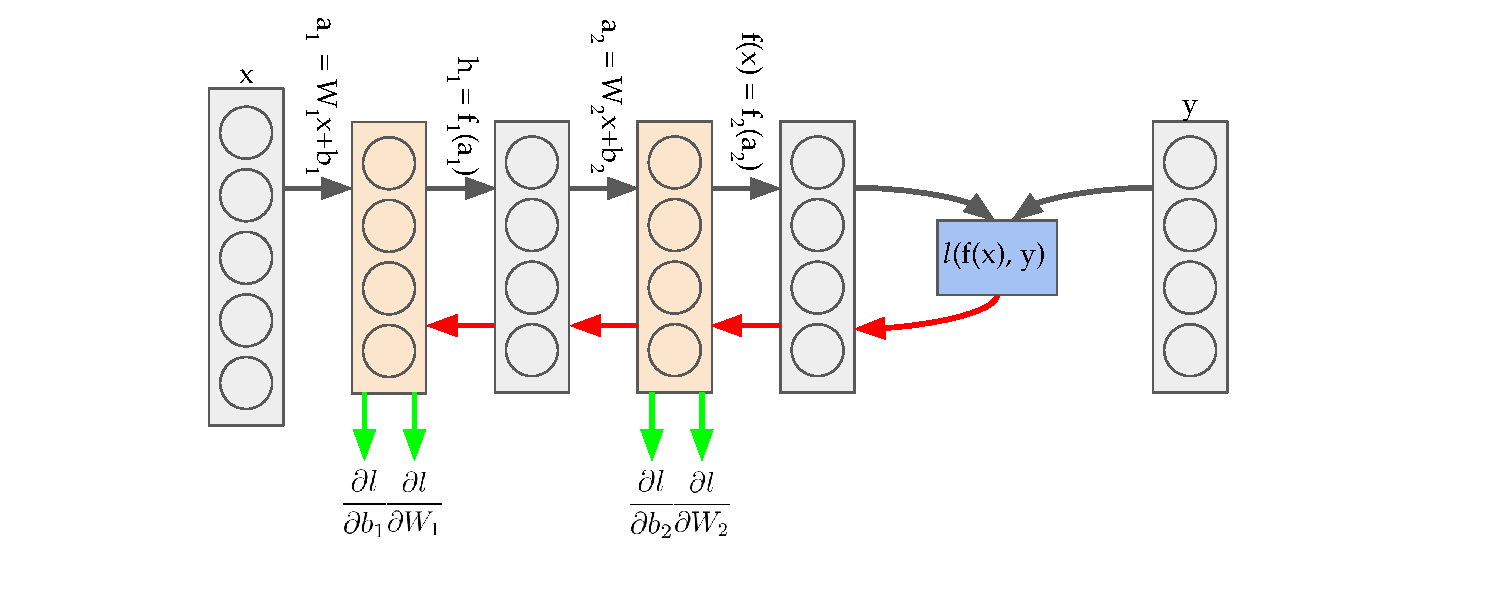
\includegraphics[width=1\textwidth]{figures/backprop}\caption{Forward (in black) and backward (in red) propagation of the intermediate
results of the process of computing the output of the network and
the gradient corresponding to this output and the desired \textquotedbl{}true\textquotedbl{}
output. The green arrows represent the computation of the gradients
with respect to the parameters, given the gradients with respect to
the pre-activations.\label{fprop-bprop}}

\end{figure}


\subsection{Automatic differentiation tools}

A key component in training neural networks is the library that we
use to implement our models. The difficulty of implementing backpropagation
in all kinds of neural networks inspired models, is solved using an
automatic differentiation tool, such as Theano \citep{bastien2012theano}.
Using such a tool we can define a model and a scalar cost function,
then call a method \texttt{grad} that takes care of building the computational
graph of all operations required to get the gradients with respect
to the parameters.

\section{Stochastic gradient descent\label{sec:Stochastic-gradient-descent}}

While backpropagation is an efficient way of computing the exact gradient
of the empirical risk with respect to the parameters, in practice
we are not required to use its exact value, but rather we can use
an estimate of the gradient, as long as this estimate will make our
objective decrease. It is worth recalling at this point that even
the exact gradient of the empirical risk is different of the real
gradient we would like to follow, which is the gradient of the true
expected risk \ref{subsec:Empirical-risk-and}.

A good estimate is obtained by computing the gradient using a smaller
subset of our dataset, called a mini-batch. Replacing the gradient
descent update with this estimate is called mini-batch gradient descent,
and the extreme case where we take a mini-batch size of 1 is called
\textbf{stochastic gradient descent} (SGD) \citep{bottou2010large}.
The main benefit of using SGD instead of full gradient descent is
that we can reduce the memory required to compute the gradient, in
order to fit in the memory of a GPU, which is very efficient for computing
vector operations such as the one required to get the values of our
gradients. The memory required to backpropagate the intermediate gradients
(red arrows in figure \ref{fprop-bprop}) is proportional to the size
of the mini-batch, and so we face a trade-off between obtaining a
noisier update direction with a small mini-batch, but very fast, and
obtaining a direction that is more precise but that takes longer.
Typically it is more efficient to compute several noisy gradients
using mini-batches that in the GPU memory and make several updates,
than to compute a single more precise update on a bigger mini-batch
or the full dataset.

\section{Hyperparameters}

In the preceding sections we have introduced the learning rate (section
\ref{sec:Gradient-descent-and}) and the minibatch size (section \ref{sec:Stochastic-gradient-descent}).
These values are called hyperparameters, which is another kind of
parametrization of our learning procedure. Hyperparameters also include
the structure of our model, such as the number of hidden layers and
hidden units, the number of training iterations, the coefficients
of the regularization terms. The success of our learning procedure
is dependant on the values of the hyperparameters. We do not find
the optimal value using gradient descent, but instead we tune it by
running several time the same experiment with different hyperparameter
values, and compare the final value of the risk. 

A difficulty in comparing optimization algorithms resides in the fact
that there performances can change drastically for different values
of hyperparameters. Optimization papers sometimes mention heuristics
that they experimentally found provide with a sensible value for some
hyperparameters. But to overcome this difficulty and provide ``fair''
benchmarks, we usually tune the values of the hyperparameters by trying
several sets of values. Hyperparameters tuning is a research field
on its own, so we will just introduce 2 existing methods and we will
later motivate our use of a new technique that we call biased random
search (section \ref{biased-random-search}).

The most simple hyperparamater tuning procedure, called \textbf{grid
search}, consists in selecting values at fixed length intervals, or
using a logarithmic scale. A simple example would be a training procedure
involving only one hyperparameter: the learning rate. We can launch
several experiments for all values in $\left\{ 10^{-3},10^{-2},10^{-1},1\right\} $
for a fixed number of updates and select the learning rate for which
we obtained the best value for our target criteria such as the validation
loss. When generalizing to several hyperparameters, we have to select
all combinations of values, which make our search space grow exponentially,
and similarly for the number of experiments we will have to run.

A first extension to grid search replaces the fixed length intervals
by random samples in our search space. It is called \textbf{random
search}. Its main advantage over grid search shows up when any hyperparameters
has no important effect on the learning algorithm \citep{bergstra2012random}.
It will explore more different values for the other hyperparameters.
In this case, it clearly appears that they are correlated, in the
sense that the best value for one hyperparameter depends on the chosen
value for the other hyperparameter.

In the rest of this work, we will use an extension of random search
that we call \textbf{biased random search}, and that we present in
section \ref{biased-random-search}.

To give a more intuitive understanding of the effect of the hyperparameter
values on the learning algorithm, we also introduce a graphical representation
that helps making sense of the interaction between different hyperparameters,
which we now describe. We launch a hyperparameter search on 2 hyperparameters
and plot this point on a scatter plot, with a color scale depicting
the final result of each experiment. By observing this plot, we can
identify 2d patterns of the link between 2 hyperparameters. As an
illustration, we use the task described in section \ref{sec:autoencoder-benchmark},
using standard stochastic gradient descent and by keeping all hyperparameters
values fixed, that is we use a fixed mini-batch size, and a fixed
number of parameter updates. We tune 2 hyperparameters: the learning
rate and the variance of the initial random weights, and we plot the
result in figure \ref{fig:Relation-between-2}. These plots show the
interaction between 2 hyperparameters. We observe that the best values
lie in a region with a very particular shape that can be assimilated
to a tilted valley (it is not parallel to the x-axis nor the y-axis).

These plots and this random search technique are a key component for
assessing the true performance of optimization techniques that we
present in section 4 and 5. Indeed it is easy to experimentally find
that a new optimization technique gives better performance than a
baseline if we spend too much time tuning hyperparameters for our
new technique but stick to default values for baselines.

\begin{figure}

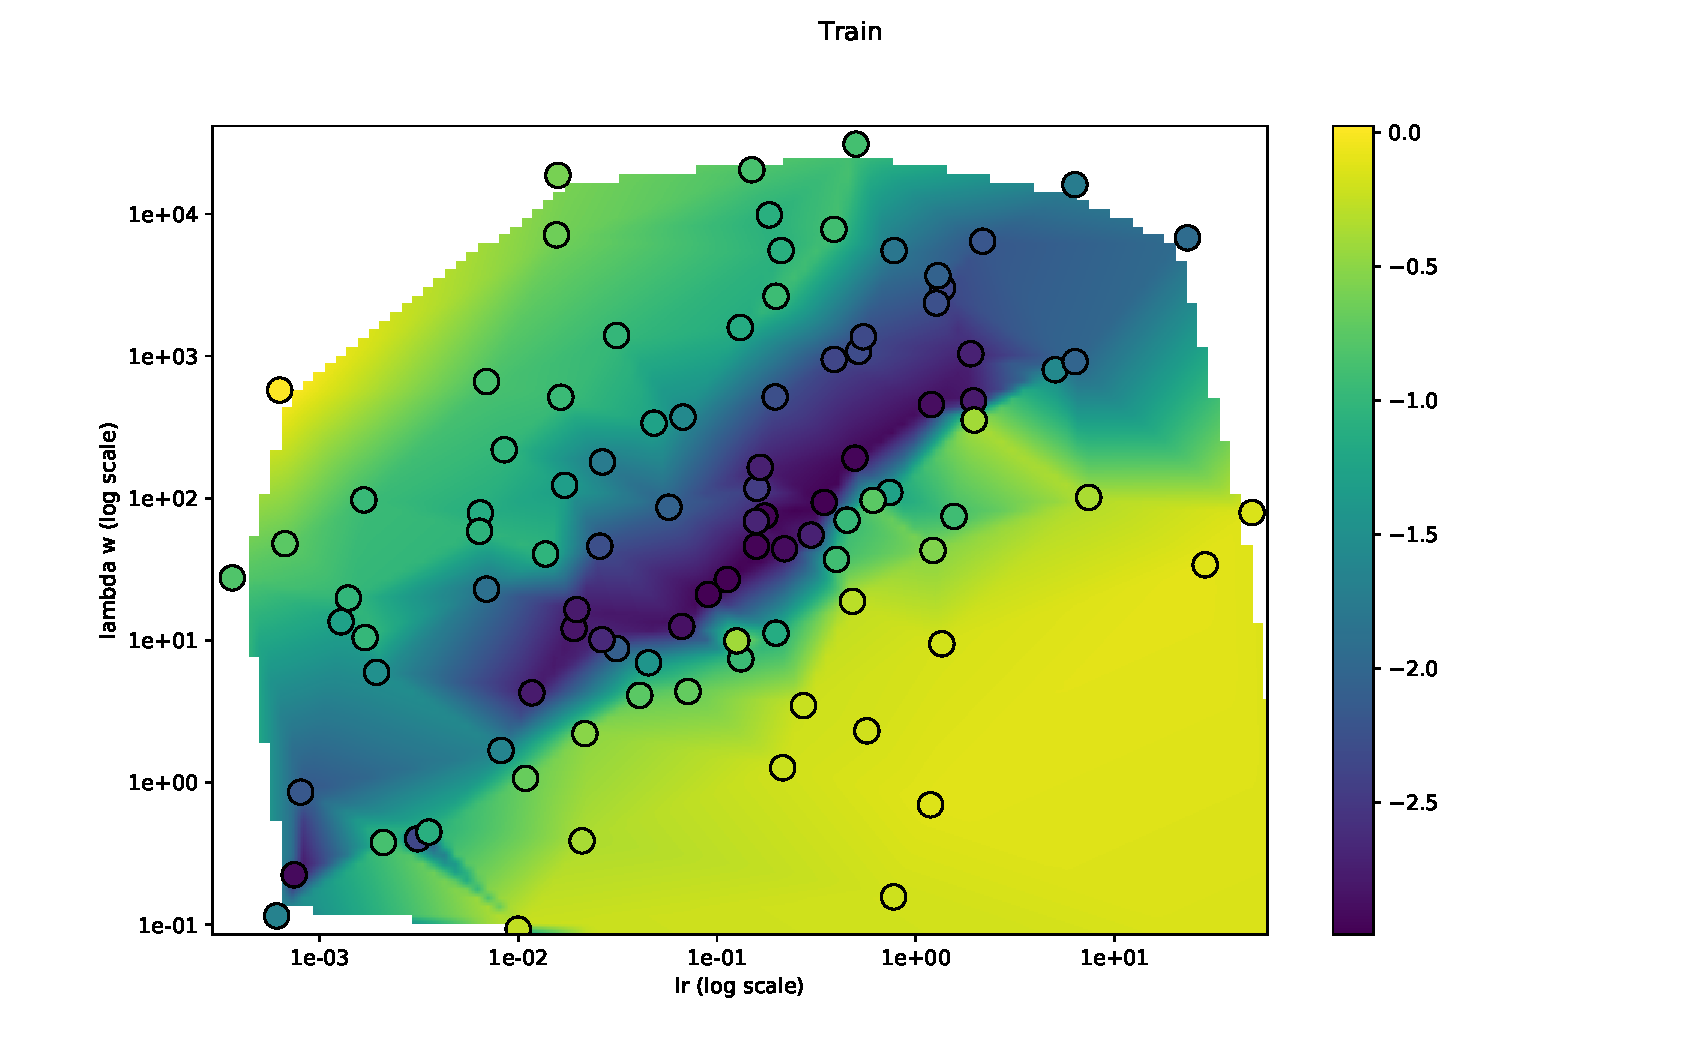
\includegraphics[width=1\textwidth]{figures/hp_search_correl}

\caption{Relation between 2 hyperparameters: for this experiment we can clearly
see that the plotted hyperparameters are not independant one from
each other. The color scale represents the final performance (best
performing runs in blue).\label{fig:Relation-between-2}}

\end{figure}


\section{Limits of (stochastic) gradient descent and some directions to overcome
them}

We can think of the task of training a neural network as the one of
finding the minimum of a scalar field in $n$ dimensions, $n$ being
the number of parameters. Each gradient descent step is a small shift
in this field. We must ensure that this path in the field of the empirical
risk is feasible. We now present reasons that can make this field
have a pathological structure, and directions to avoid these difficulties.

\subsection{Gradient magnitudes}

A common issue for deep networks or recurrents networks is how to
control the magnitude of the gradient flow for many layers. If the
jacobians $\left(\mathbf{J}_{a_{l}}^{h_{l-1}}\right)^{T}\left(\mathbf{J}_{h_{l}}^{a_{l}}\right)^{T}$
have a spectral norm that is too big, then the gradient will become
bigger and bigger for lower layers. This can happen if the weight
matrices have singular values that are too big compared to $1$, or
if the derivatives of the activation functions take big values. In
this case, we are in a situation of exploding gradients. This effect
is amplified in recurrent networks, where the same weight matrix is
repeatedly used in the backward pass. For such a ill-conditioned problem,
gradient descent will not be effective. Indeed, in the case of exploding
gradient, two layers separated by several others will have updates
of different order of magnitude.

This effect can be mitigated using gradient clipping \citep{pascanu2013difficulty}.
We can also use second order methods to compensate for gradient vanishing/exploding
as proposed in \citep{martens2011learning}.

\subsection{Initialization\label{initialization-of-weights}}

Initialization of the weight matrices is of crucial importance. In
terms of our empirical risk field in the space of parameters, it controls
how far we start from a minimum. A good initialization scheme must
at least make sure that there is enough signal flowing in forward
and backward direction, that is: the weights must be chosen not too
small, otherwise the forward signal will be smaller and smaller, and
in the meantime the weights must not be too big, so as to avoid exploding
gradients in the backward pass, and saturating functions in the forward
pass.

The most common initialization scheme at the time of writing are Glorot
initialization \citep{glorot2010understanding} and He initialization
\citep{he2015delving}. Glorot takes care of maintaining a training
signal during the forward pass, and the backward pass, by sampling
random weights from an uniform distribution with variance $\frac{\alpha}{n_{in}+n_{out}}$,
while He argues that only the forward pass matters so the weights
should be initialized from a distribution with variance $\frac{\alpha}{n_{in}}$.
In both cases, $\alpha$ depends on the activation function, and the
papers propose default values for sigmoid and ReLU \citep{glorot2011deep}.
In our experiments, we treated $\alpha$ as a hyperparameter, and
tuned it using a biased random search (section \ref{biased-random-search}).

\subsection{Gradient smoothing methods}

A family of optimization tricks use geometrical considerations in
the space of parameter values. In this case with some common sense
we can define a simple principle to derive better updates which is
that for an equivalent decrease of the empirical risk, we must follow
a direction of descent that has a smaller derivative for longer in
order to achieve the same improvement as for a direction that has
a larger derivative. Many popular techniques use this principle, the
most successful ones at the time of writing being Adam \citep{kingma2014adam},
RMSProp \citep{tieleman2012lecture}, Nesterov momentum \citep{nesterov1983method}
and so on.

\chapter{Second order methods in neural networks}

In this section, we introduce the well known second order methods
known as Newton's method and the less popular but very effective natural
gradient descent. We then derive the updates of this methods adapted
to neural networks.

\section{Second order methods}

\subsection{Newton steps}

Second order methods refer to all optimization methods that make use
of the second derivative or Hessian matrix of the function to be minimized.
It follows from the Taylor series decomposition of the function:

\begin{eqnarray*}
f\left(x+\Delta x\right) & = & f\left(x\right)+\left(\nabla f\right)_{x}^{T}\Delta x+\frac{1}{2}\Delta x^{T}\left(\nabla^{2}f\right)_{x}\Delta x+o\left(\left\Vert \Delta x\right\Vert _{2}^{2}\right)
\end{eqnarray*}

$\left(\nabla^{2}f\right)_{x}$ is the Hessian matrix of $f$, expressed
at $x$. We use the little-o notation $o$ that represents an unknown
function with the only property that $\lim_{x\rightarrow0}\frac{o\left(x\right)}{x}=0$.
By constraining $\left\Vert \Delta x\right\Vert _{2}^{2}$ too stay
small, we can ignore higher order terms ($o\left(\left\Vert \Delta x\right\Vert _{2}^{2}\right)=0$)
and we have a quadratic approximation for $f$. Using this approximation
in a minimization problem, we get the following minimization which
has a closed form solution:

\begin{eqnarray*}
\Delta x^{*} & = & \text{argmin}_{\Delta x}f\left(x+\Delta x\right)\\
 & \approx & \text{argmin}_{\Delta x}f\left(x\right)+\left(\nabla f\right)_{x}^{T}\Delta x+\frac{1}{2}\Delta x^{T}\left(\nabla^{2}f\right)_{x}\Delta x
\end{eqnarray*}

This expression is solved by taking the derivative with respect to
$\Delta x$, and setting it to zero which yields:

\begin{eqnarray*}
\left(\nabla^{2}f\right)_{x}\Delta x & = & -\left(\nabla f\right)_{x}
\end{eqnarray*}

If we assume that $f$ has a minimum in $x^{*}$, then the Hessian
will be positive definite in $x^{*}$, and under the supplementary
assumption that the Hessian is continuous, it will also be positive
definite in a neighborhood of $x^{*}$. In this case, it is invertible
and we get the solution:

\begin{eqnarray}
\Delta x & = & -\left(\nabla^{2}f\right)_{x}^{-1}\left(\nabla f\right)_{x}\label{eq:newton-step}
\end{eqnarray}

This update \ref{eq:newton-step} is called the \textbf{Newton step}.
By making several iterations of Newton, and under the assumption that
we are close enough to a minimum, the updates will converge to it.

The main difficulty of this algorithm is that it does not scale well
when applied to problems with many variables such as neural network
optimization. In this case $f$ is the empirical risk, and the variables
that we are optimizing are the parameters of the network. The limitations
come from the following aspects:
\begin{enumerate}
\item \textit{Getting the value of the Hessian matrix}: Using an automatic
differentiation software, we can get an expression for the Hessian,
by differentiating the symbolic expression of the gradient. But unlike
the computation of the gradient, the graph produced to compute the
Hessian will have much more nodes. We will explore this question in
more details in section \ref{subsec:gauss-newton} and present an
approximate value of the Hessian called Gauss-Newton.
\item \textit{Storing the Hessian matrix}: The Hessian matrix is a square
matrix of size $n_{\text{parameters}}\times n_{parameters}$. As the
number of parameters grows, which is the case when building deep networks,
the memory required to store the Hessian will grow in $O\left(n^{2}\right)$.
We will present an approximation of the Hessian that saves memory
in section \ref{subsec:Block-diagonal-Hessian}.
\item \textit{Inverting the Hessian matrix}: Inverting the Hessian matrix
is also costly as it grows in $O\left(n^{3}\right)$ with the size
of the matrix. Some techniques use 2nd order information without inverting
the Hessian such as \textit{Hessian Free} \citep{martens2010deep}.
We propose to factorize the Hessian so as to require inverting a smaller
matrix while benefiting from some 2nd order information in section
\ref{subsec:focus-covariance}.
\end{enumerate}

\subsection{The learning rate\label{subsec:The-learning-rate}}

Amongst other hyperparameters, the learning rate of standard (stochastic)
gradient descent plays a particular role which we will show in the
following. We use the quadratic approximation for a function $f$:

\begin{eqnarray*}
\Delta x^{*} & = & \text{argmin}_{\Delta x}f\left(x\right)+\left(\nabla f\right)_{x}^{T}\Delta x+\frac{1}{2}\Delta x^{T}\left(\nabla^{2}f\right)_{x}\Delta x+o\left(\left\Vert \Delta x\right\Vert _{2}^{2}\right)
\end{eqnarray*}

If we replace the Hessian with a scaled diagonal matrix $\lambda\mathbf{I}$,
we can simplify this expression to the following one that is often
used for deriving the first order gradient descent update:

\begin{eqnarray*}
\Delta x^{*} & \approx & \text{argmin}_{\Delta x}f\left(x\right)+\left(\nabla f\right)_{x}^{T}\Delta x+\frac{\lambda}{2}\Delta x^{T}\Delta x
\end{eqnarray*}

By solving this minimization problem we recover the update $\Delta x^{*}=-\frac{1}{\lambda}\left(\nabla f\right)_{x}$
with $\frac{1}{\lambda}$ playing the role of the usual learning rate.
But of course this $\lambda$ hides second order information. In fact,
\citet{lecun1993automatic} proposes to automatically adapt the value
of the learning rate by using the biggest eigenvalue of the hessian
as $\lambda$. In this case we are guaranteed that we do not go too
far in the direction of greatest curvature (which is the corresponding
eigenvector). But in exchange it will equivalently scale down an update
in any other direction, even if an optimal step would require to go
further in this direction.

\subsection{Validity of Newton for non quadratic functions and Tikhonov regularization\label{tikhonov}}

In the previous section, we considered that our function was approximated
by its second order Taylor series decomposition. While this is true
in a neighborhood of $x$, the approximation becomes less precise
as we move away from $x$. In particular this is the case when the
Newton step provide big updates, that is when the Hessian has at least
one small eigenvalue. The corresponding eigenvector points in a direction
that will have a low curvature using the quadratic approximation,
so the minimum following this direction will be far away. But the
actual function that we are minimizing is not a quadratic, and the
terms hidden in $o\left(\left\Vert \Delta x\right\Vert _{2}^{2}\right)$
will become preponderant for bigger values of $\Delta x$.

To counter this undesirable effect, we simply add a regularization
term that penalizes bigger values of $\Delta x$:

\begin{eqnarray*}
\Delta x^{*} & = & \text{argmin}_{\Delta x}f\left(x+\Delta x\right)\\
 & \approx & \text{argmin}_{\Delta x}f\left(x\right)+\left(\nabla f\right)_{x}^{T}\Delta x+\frac{1}{2}\Delta x^{T}\left(\nabla^{2}f\right)_{x}\Delta x+\frac{\epsilon}{2}\left\Vert \Delta x\right\Vert _{2}^{2}\\
 & = & \text{argmin}_{\Delta x}\left(\nabla f\right)_{x}^{T}\Delta x+\frac{1}{2}\Delta x^{T}\left(\left(\nabla^{2}f\right)_{x}+\epsilon\mathbf{I}\right)\Delta x
\end{eqnarray*}

This gives the Tikhonov regularized version of the Newton step:

\begin{eqnarray*}
\Delta x & = & -\left(\left(\nabla^{2}f\right)_{x}+\epsilon\mathbf{I}\right)^{-1}\left(\nabla f\right)_{x}
\end{eqnarray*}

This new hyperparameter $\epsilon$ controls the size of the steps,
and thus plays a very similar role to the learning rate.

In addition to this, we can also mention that it stabilizes the inversion
when the condition number of $\left(\nabla^{2}f\right)_{x}$ is too
big, and that it can account for the estimation error when we estimate
$\left(\nabla^{2}f\right)_{x}$ using a minibatch of examples instead
of using the true risk.

\subsection{Gauss-Newton approximation of the Hessian\label{subsec:gauss-newton}}

In the case of neural network optimization, the Hessian matrix we
need to evaluate is the second derivative of the empirical risk, with
respect to the parameters. A first remark that we can make, is that
it is also composed of a sum of second order derivatives, to be computed
at each example of the dataset:

\begin{eqnarray*}
\mathbf{H} & = & \frac{\partial^{2}R}{\partial\theta^{2}}\\
 & = & \frac{\partial^{2}}{\partial\theta^{2}}\left\{ \frac{1}{n}\sum_{i}l\left(f_{\theta}\left(x_{i}\right),y_{i}\right)\right\} \\
 & = & \frac{1}{n}\sum_{i}\frac{\partial^{2}}{\partial\theta^{2}}\left\{ l\left(f_{\theta}\left(x_{i}\right),y_{i}\right)\right\} 
\end{eqnarray*}

By making use of the chain rule we can also give an expression for
the second derivative of the loss, for a single example. We start
with the first derivative:

\begin{eqnarray*}
\frac{\partial}{\partial\theta}\left\{ l\left(f_{\theta}\left(x_{i}\right),y_{i}\right)\right\}  & = & \mathbf{J}_{\theta}\left(x_{i},\theta\right)^{T}\left(\frac{\partial}{\partial f}\left\{ l\left(f_{\theta}\left(x_{i}\right),y_{i}\right)\right\} \right)^{T}
\end{eqnarray*}

$\mathbf{J}$ is the jacobian of the output of the network $f$ with
respect to the parameters $\theta$. In this notation we made the
dependance in $\theta$ of both parts of the product explicit. Note
that both parts also take different values for each examples $x_{i}$.
We now derive this expression once more to obtain the Hessian:

\begin{eqnarray*}
\frac{\partial^{2}}{\partial\theta^{2}}\left\{ l\left(f\left(x_{i},\theta\right),y_{i}\right)\right\}  & = & \underbrace{\mathbf{J}_{\theta}\left(x_{i},\theta\right)^{T}\frac{\partial^{2}}{\partial f^{2}}\left\{ l\left(f_{\theta}\left(x_{i}\right),y_{i}\right)\right\} \mathbf{J}_{\theta}\left(x_{i},\theta\right)}_{G_{f}\left(x_{i},\theta\right)}\\
 &  & +\sum_{j}\left(\nabla^{2}f_{\theta}\left(x_{i}\right)_{j}\right)\left(\frac{\partial}{\partial f_{j}}\left\{ l\left(f_{\theta}\left(x_{i}\right),y_{i}\right)\right\} \right)^{T}
\end{eqnarray*}

$G_{f}\left(x_{i},\theta\right)$ is called the Gauss-Newton (GN)
approximation of the Hessian \citep{schraudolph2002fast}. The remainder
is proportional to $\frac{\partial}{\partial f_{j}}\left\{ l\left(f_{\theta}\left(x_{i}\right),y_{i}\right)\right\} $.
As we get closer to the the optimum, this part will go toward $0$
as it is a first derivative, so the approximation will get more precise.
At a minimum for $l\left(f_{\theta}\left(x_{i}\right),y_{i}\right)$,
we will have $\frac{\partial^{2}}{\partial\theta^{2}}\left\{ l\left(f_{\theta}\left(x_{i}\right),y_{i}\right)\right\} =G_{f}\left(x_{i},\theta\right)$
so it is a reasonable approximation to use in practice. Note that
a minimum for the empirical risk $R\left(\theta\right)$ will not
necessarily be a minimum for each example $l\left(f_{\theta}\left(x_{i}\right),y_{i}\right)$,
especially if the capacity of the neural network is not sufficient
to model the data distribution.

In terms of computational cost, we can also note that we can compute
the GN part using standard backpropagation, but this time of the jacobian.
The other term is much more complicated because it involves a second
derivative of a composed function.

In practice, $G_{f}\left(x_{i},\theta\right)$ presents a much more
convenient expression for common loss functions, as the second derivative
of the loss with respect to the ouput of the network simplifies (table
\ref{gn-loss}).

\begin{table}
\begin{tabular}{|r|c|}
\hline 
Loss function & $\frac{\partial^{2}}{\partial f_{\theta}^{2}}\left\{ l\left(f_{\theta}\left(x_{i}\right),y_{i}\right)\right\} $\tabularnewline
\hline 
\hline 
quadratic error & $\mathbf{I}$\tabularnewline
cross entropy for binary decision & $\frac{y_{i}}{\left(f_{\theta}\left(x_{i}\right)\right)^{2}}+\frac{1-y_{i}}{\left(1-f_{\theta}\left(x_{i}\right)\right)^{2}}$\tabularnewline
cross entropy for multiclass classification & $\text{diag}\left(\frac{y_{i}}{\left(f_{\theta}\left(x_{i}\right)\right)^{2}}\right)$\tabularnewline
\hline 
\end{tabular}

\caption{\label{gn-loss}Expressions for the Gauss-Newton approximation of
the Hessian, for a single example $x_{i}$. For the cross entropy,
all operations (division, squarred value) are elementwise, and the
$\text{diag}$ function transforms a vector into a diagonal matrix
with the vector values on its diagonal. Full derivation in appendix.}
\end{table}

We finally give an expression for the Gauss-Newton approximation of
the Hessian for the empirical risk:

\begin{eqnarray*}
G_{f}\left(\theta\right) & = & \frac{1}{n}\sum_{i}\mathbf{J}_{\theta}\left(x_{i},\theta\right)^{T}\frac{\partial^{2}}{\partial f^{2}}\left\{ l\left(f_{\theta}\left(x_{i}\right),y_{i}\right)\right\} \mathbf{J}_{\theta}\left(x_{i},\theta\right)
\end{eqnarray*}

We will show in section \ref{sec:Decomposition-using-the} that this
matrix can be factorized to design optimization algorithms adapted
to the particular structure of neural networks.

\subsection{Block diagonal Hessian \label{subsec:Block-diagonal-Hessian}}

Apart from the issue of computing a value for the hessian matrix,
a main limit is that we need to invert it. The hessian matrix has
size $n_{\text{parameters}}\times n_{\text{parameters}}$, and the
procedure used for numerically inverting a square matrix requires
$O\left(n^{3}\right)$ operations so it rapidly becomes untractable
for deep networks. A first approximation we make is by ignoring the
interactions between the parameters of different layers. We make the
hessian block diagonal, each block having the size of the number of
parameters of the corresponding layer. An interesting property of
block diagonal matrices is that we get the inverse by inverting every
smaller block separately:

\begin{eqnarray*}
\left(\nabla^{2}f\right)^{-1} & \approx & \left(\begin{array}{cccc}
\mathbf{H}_{1} & 0 & \cdots & 0\\
0 & \mathbf{H}_{2} &  & \vdots\\
\vdots &  & \ddots & 0\\
0 & \cdots & 0 & \mathbf{H}_{n}
\end{array}\right)^{-1}=\left(\begin{array}{cccc}
\mathbf{H}_{1}^{-1} & 0 & \cdots & 0\\
0 & \mathbf{H}_{2}^{-1} &  & \vdots\\
\vdots &  & \ddots & 0\\
0 & \cdots & 0 & \mathbf{H}_{n}^{-1}
\end{array}\right)
\end{eqnarray*}

It also makes the implementation easier, as we can treat each block
``locally'' in the network, and use its inverse to update the gradient
direction for the corresponding block (or layer) using $\theta_{i}\leftarrow\theta_{i}-\lambda\mathbf{H}_{i}^{-1}\frac{\partial C}{\partial\theta_{i}}$.
We do not need to store a big $n_{\text{parameters}}\times n_{\text{parameters}}$
matrix.

\section{Natural gradient methods}

We now present the natural gradient. We give some context and interpration
for the natural gradient, and we give its expression for neural networks.

\subsection{Fisher Information Matrix}

The Fisher information matrix (FIM) is well used in statistics. In
the context of machine learning, and in particular deep learning,
we use its inverse as a preconditioner for the gradient descent algorithm,
similarly to the Newton algorithm (section \ref{eq:newton-step}).
In this section, we show how the FIM can be derived from the KL divergence
and how we get a better ``natural'' gradient using this information.
Let us first write the definition of the KL divergence for 2 distributions
$p$ and $q$:

\begin{eqnarray*}
\text{KL}\left(p\parallel q\right) & = & \mathbb{E}_{p}\left[\log\left(\frac{p}{q}\right)\right]
\end{eqnarray*}

From a broad view, it is a non-negative quantity that measures how
much $q$ differs from $p$. In particular, $\text{KL}\left(p\parallel q\right)=0$
when $p=q$. Note that it is not symmetric, so it cannot be considered
a true metric. We now use the probabilistic interpretation of neural
networks, and consider that the examples from a dataset are drawn
from a joint distribution $p_{\theta}\left(x,y\right)=p_{\theta}\left(y|x\right)p\left(x\right)$
where $p_{\theta}\left(y|x\right)$ is the function that we model
with the neural network, and $p\left(x\right)$ is the input distribution.

One can view natural gradient as using KL divergence as a regularizer
when doing gradient descent. We will denote by $p_{\theta}\left(x,y\right)$
a parametric model and $\Delta\theta$ a change in its parameter values.
$\text{KL}\left(p_{\theta}\left(x,y\right)\parallel p_{\theta+\Delta\theta}\left(x,y\right)\right)$
is used as our regularizer, so that each change $\Delta\theta$ gives
a desired change magnitude in the distribution space that we control
using a new hyperparameter. Instead of using the full expression for
$\text{KL}\left(p_{\theta}\left(x,y\right)\parallel p_{\theta+\Delta\theta}\left(x,y\right)\right)$
we will use its second order Taylor series around $\theta$ (for full
derivation see for instance \citet{pascanu2013revisiting}):

\begin{eqnarray*}
\text{KL}\left(p_{\theta}\left(x,y\right)\Vert p_{\theta+\Delta\theta}\left(x,y\right)\right) & = & \Delta\theta^{T}\mathbf{F}\Delta\theta+o(\left\Vert \Delta\theta\right\Vert _{2}^{2})
\end{eqnarray*}

$\mathbf{F}=\mathbb{E}_{p_{\theta}\left(x,y\right)}\left[\left(\frac{\partial\log p_{\theta}\left(x,y\right)}{\partial\theta}\right)^{T}\left(\frac{\partial\log p_{\theta}\left(x,y\right)}{\partial\theta}\right)\right]$
is the Fisher information matrix (FIM), which can be used directly
as a regularizer as we shall see shortly. Interestingly, even if the
KL divergence is not symmetric, its second order approximation is,
as we also have $\text{KL}\left(p_{\theta+\Delta\theta}\Vert p_{\theta}\right)=\Delta\theta^{T}\mathbf{F}\Delta\theta+o(\left\Vert \Delta\theta\right\Vert _{2}^{2})$
(note that we swapped the terms in the KL).

\subsection{Natural gradient descent}

As noted in section \ref{subsec:The-learning-rate}, the parameter
update vector used in ordinary gradient descent can be otabined as
the result of the following minimization problem:

\begin{eqnarray*}
\Delta\theta^{*} & = & \text{argmin}_{\Delta\theta}\Delta\theta^{T}\nabla_{\theta}R+\frac{1}{2\lambda}\Delta\theta^{T}\Delta\theta
\end{eqnarray*}

where $R$ is the empirical risk, as previously defined in eq \ref{eq:empirical-risk}
in section \ref{subsec:Empirical-risk-and}.

This expression can be easily solved giving the usual gradient descent
update $\Delta\theta=-\lambda\nabla_{\theta}R$. The parameter $\lambda$
is the usual learning rate, and controls how much each parameter can
change. We will now add a new regularizer using the FIM, and transform
the minimization problem into:

\begin{eqnarray*}
\Delta\theta^{*} & = & \text{argmin}_{\Delta\theta}\Delta\theta^{T}\nabla_{\theta}R+\frac{1}{2\lambda}\Delta\theta^{T}\Delta\theta+\frac{1}{2\epsilon}\Delta\theta^{T}\mathbf{F}\Delta\theta
\end{eqnarray*}

We now constrain our gradient step to be small in term of change of
parameter values, and also to be small in term of how much the resulting
distribution changes. This expression can be solved to give $\Delta\theta^{*}=-\lambda\left(\mathbf{I}+\frac{\lambda}{\epsilon}\mathbf{F}\right)^{-1}\nabla_{\theta}R$.
This expression also gives an insight for the role of $\lambda$ and
$\epsilon$, which control 2 different but related quantities expressed
by our constraints. This new update is called the natural gradient
\citep{amari1998natural}.

\subsection{An expression for the FIM using jacobians}

Using the probabilistic interpretation of neural networks, the FIM
can be expressed $\mathbf{F}=\mathbb{E}_{p_{\theta}\left(x,y\right)}\left[\left(\frac{\partial\log p_{\theta}\left(x,y\right)}{\partial\theta}\right)^{T}\left(\frac{\partial\log p_{\theta}\left(x,y\right)}{\partial\theta}\right)\right]$
which simplifies in:

\begin{eqnarray*}
\mathbf{F} & = & \mathbb{E}_{p_{\theta}\left(x,y\right)}\left[\left(\frac{\partial\log p_{\theta}\left(x,y\right)}{\partial\theta}\right)^{T}\left(\frac{\partial\log p_{\theta}\left(x,y\right)}{\partial\theta}\right)\right]\\
 & = & \mathbb{E}_{x\sim p\left(x\right)}\left[\mathbb{E}_{y\sim p_{\theta}\left(y|x\right)}\left[\left(\frac{\partial\log p_{\theta}\left(x,y\right)}{\partial\theta}\right)^{T}\left(\frac{\partial\log p_{\theta}\left(x,y\right)}{\partial\theta}\right)\right]\right]
\end{eqnarray*}

Since $\log p_{\theta}\left(x,y\right)=\log p_{\theta}\left(y|x\right)+\log p\left(x\right)$
and $p\left(x\right)$ does not depend on $\theta$ then this can
be further simplified in:

\begin{eqnarray*}
\mathbf{F} & = & \mathbb{E}_{x\sim p\left(x\right)}\left[\mathbb{E}_{y\sim p_{\theta}\left(y|x\right)}\left[\left(\frac{\partial\log p_{\theta}\left(y|x\right)}{\partial\theta}\right)^{T}\left(\frac{\partial\log p_{\theta}\left(y|x\right)}{\partial\theta}\right)\right]\right]
\end{eqnarray*}

Interestingly, for the usual distributions expressed by neural networks,
we can derive an exact expression for the inner expectation. The FIM
takes the following simple form as shown by \citet{pascanu2013revisiting}:

\begin{eqnarray*}
\mathbf{F} & = & \mathbb{E}_{x\sim q\left(x\right)}\left[\mathbf{J}_{\theta}\left(x,\theta\right)^{T}D\left(f_{\theta}\left(x\right)\right)\mathbf{J}_{\theta}\left(x,\theta\right)^{T}\right]
\end{eqnarray*}

The values for $x$ are drawn from the data generating distribution
$q$. Similarly to section \ref{subsec:gauss-newton}, the notation
$\mathbf{J}_{\theta}\left(x,\theta\right)^{T}$ is used for the jacobian
of the output of the network (i.e. the probability expressed at a
given $x$ : $p\left(y\mid x\right)$), with respect to the parameters.
In other words, it measures how much the output of the network $p\left(y|x\right)$
will change for a given $x$ if we change the parameters. For usual
loss functions, $D$ is a diagonal matrix with non negative diagonal
terms, and depends of the cost function used. For the quadratic loss
it is the identity (table \ref{expressions-fisher}).

\begin{table}
\begin{tabular}{|r|c|}
\hline 
Loss function & $D\left(f_{\theta}\left(x\right)\right)$\tabularnewline
\hline 
\hline 
quadratic error & $\mathbf{I}$\tabularnewline
cross entropy for binary decision & $\frac{1}{f_{\theta}\left(x\right)\left(1-f_{\theta}\left(x\right)\right)}$\tabularnewline
cross entropy for multiclass classification & $\text{diag}\left(\frac{1}{f_{\theta}\left(x\right)}\right)$\tabularnewline
\hline 
\end{tabular}

\caption{\label{expressions-fisher}Expressions for the FIM, for a single sample
$x_{i}$. For the cross entropy, all operations (division, squarred
value) are elementwise, and the $\text{diag}$ function transforms
a vector into a diagonal matrix with the vector values on its diagonal.
Full derivation in appendix.}
\end{table}


\subsection{Approximating the FIM}

Similarly to the Hessian, the FIM is difficult to compute because
of its size ($n_{parameters}\times n_{parameters}$) and because in
general we do not have an expression for $q$ but only samples from
a training dataset. As for Newton, we can make the two following approximations:
\begin{itemize}
\item A first approximation that we can make is by ignoring the interactions
between layers. In this case the FIM takes the form of a block diagonal
matrix, where each block is a square matrix which has the size of
the parameters of a layer. For a neural network with $n_{layers}$
layers this reduces the FIM into $n_{layers}$ smaller matrices. We
will denote by $\mathbf{F}_{i}$ the block corresponding to layer
$i$.
\item A second common approximation we make in practice is to use the empirical
FIM for a training dataset of $n$ examples $x_{i}$: $\mathbf{F}=\frac{1}{n}\sum_{i}\mathbf{J}_{\theta}\left(x_{i},\theta\right)^{T}D\left(f_{\theta}\left(x\right)\right)\mathbf{J}_{\theta}\left(x_{i},\theta\right)^{T}$.
\end{itemize}

\section{Gauss-Newton and Fisher share a very similar structure}


\subsection{Relation between the FIM and the GN approximation of the Hessian}

We have just shown that the Gauss-Newton of the empirical risk with
respect to the parameters, and the Fisher Information Matrix share
a similar structure that is composed of the jacobians of the output
of the network with respect to the parameters, and a symmetric matrix:

\begin{equation}
\frac{1}{n}\sum_{i}\mathbf{J}_{\theta}\left(x_{i},\theta\right)^{T}D\left(f_{\theta}\left(x_{i}\right)\underbrace{,y_{i}}_{\text{opt}}\right)\mathbf{J}_{\theta}\left(x_{i},\theta\right)^{T}\label{eq:general_form}
\end{equation}
The main difference is in this symmetric matrix $D\left(f_{\theta}\left(x\right),y\right)$.
For Fisher methods it does not depend on any true target and it is
just an intrinsic property of a neural network, associated with an
input distribution. We can thus remove the $y$: $D\left(f_{\theta}\left(x\right)\right)$.
In the case of the GN matrix it depends on the true target $y$ in
general, with a notable exception for the quadratic error.

\begin{table}[h]
\begin{tabular}{|r|c|c|}
\cline{2-3} 
\multicolumn{1}{r|}{} & Gauss-Newton & Fisher\tabularnewline
\multicolumn{1}{r|}{} & $D\left(f_{\theta}\left(x\right),y\right)$ & $D\left(f_{\theta}\left(x\right)\right)$\tabularnewline
\hline 
quadratic error & $\mathbf{I}$ & $\mathbf{I}$\tabularnewline
cross entropy for binary decision & $\frac{y_{i}}{\left(f_{\theta}\left(x_{i}\right)\right)^{2}}+\frac{1-y_{i}}{\left(1-f_{\theta}\left(x_{i}\right)\right)^{2}}$ & $\frac{1}{f_{\theta}\left(x\right)\left(1-f_{\theta}\left(x\right)\right)}$\tabularnewline
cross entropy for multiclass classification & $\text{diag}\left(\frac{y_{i}}{\left(f_{\theta}\left(x_{i}\right)\right)^{2}}\right)$ & $\text{diag}\left(\frac{1}{f_{\theta}\left(x\right)}\right)$\tabularnewline
\hline 
\end{tabular}

\caption{\label{gn-fim}Expressions for the middle term $D\left(f_{\theta}\left(x\right),y\right)$
and $D\left(f_{\theta}\left(x\right)\right)$ for GN and FIM}
\end{table}


\subsection{An original interpretation from the output of the network}

In the cases where $D$ is a diagonal matrix (i.e. cross entropy and
quadratic error, see eq \ref{eq:general_form} and table \ref{gn-fim}),
we can rewrite both GN and FIM matrices applied to an update as a
norm in the space of the output of the network:

\begin{eqnarray*}
\Delta\theta^{*} & = & \underset{\Delta\theta}{\text{argmin}}\left(\nabla R\right)_{\theta}^{T}\Delta\theta+\frac{1}{2}\Delta\theta^{T}\frac{1}{n}\sum_{i}\mathbf{J}_{\theta}\left(x_{i},\theta\right)^{T}D\left(f\left(x_{i},\theta\right),y_{i}\right)\mathbf{J}_{\theta}\left(x_{i},\theta\right)\Delta\theta+\frac{1}{2\lambda}\Delta\theta^{T}\Delta\theta\\
 & = & \underset{\Delta\theta}{\text{argmin}}\left(\nabla R\right)_{\theta}^{T}\Delta\theta+\frac{1}{2}\frac{1}{n}\sum_{i}\left\langle D\left(f\left(x_{i},\theta\right),y_{i}\right)\mathbf{J}_{\theta}\left(x_{i},\theta\right)\Delta\theta,\mathbf{J}_{\theta}\left(x_{i},\theta\right)\Delta\theta\right\rangle +\frac{1}{2\lambda}\Delta\theta^{T}\Delta\theta\\
 & = & \underset{\Delta\theta}{\text{argmin}}\left(\nabla R\right)_{\theta}^{T}\Delta\theta+\frac{1}{2}\frac{1}{n}\sum_{i}\left\langle D\left(f\left(x_{i},\theta\right),y_{i}\right)\Delta f_{\theta}\left(x_{i},\Delta\theta\right),\Delta f_{\theta}\left(x_{i},\Delta\theta\right)\right\rangle +\frac{1}{2\lambda}\Delta\theta^{T}\Delta\theta
\end{eqnarray*}

We denoted by $\Delta f_{\theta}\left(x_{i},\Delta\theta\right)=\mathbf{J}_{\theta}\left(x_{i},\theta\right)\Delta\theta$
a first order approximation of the change in the value of $f_{\theta}\left(x_{i}\right)$
induced by a change $\Delta\theta$ of $\theta$ for example $x_{i}$.
With this decomposition we can understand GN and natural gradient
as being a regularizer for each example, using the metrics $D\left(f\left(x_{i},\theta\right),y_{i}\right)$
that depends on the considered example. We regularize for several
undesirable effect:
\begin{itemize}
\item We ensure that$\Delta f_{\theta}\left(x_{i},\Delta\theta\right)$
cannot take a large value. This distributes the effect of the update
evenly between examples, instead of having a large change in $f_{\theta}\left(x_{i}\right)$
for a single example, and smaller changes for others.
\item We weight this changes using $D\left(f\left(x_{i},\theta\right),y_{i}\right)$.
For the cross entropies for instance we observe that this term grows
with $\frac{1}{f_{\theta}\left(x\right)}$ (the vector of probabilities
of each class). If this vector is not evenly distributed, that is
if for one class $t$ we have a larger value of $\left(f_{\theta}\left(x\right)\right)_{t}$,
all other values will be close to $0$, which means that $\left(\frac{1}{f_{\theta}\left(x\right)}\right)_{i\neq t}$
will take a very large value. In this case we put more weight on the
examples for which our model is more confident of its prediction.
\end{itemize}

\section{A cheaper Gauss-Newton matrix for cross-entropy\label{sec:gn-trick-cheap}}

We now present a computational trick for computing the Gauss-Newton
in the case of cross-entropy. Interestingly, in the expression of
Gauss-Newton for log losses we have the unexpected equivalence $\left(\frac{\partial^{2}l}{\partial f_{\theta}^{2}}\right)_{tt}=-\left(\frac{\partial l}{\partial f_{\theta}}\right)_{t}^{2}$
for the true class $t$ and $\left(\frac{\partial^{2}l}{\partial f_{\theta}^{2}}\right)_{ii}=0=-\left(\frac{\partial l}{\partial f_{\theta}}\right)_{t}^{2}$
when $i\neq t$:

\begin{eqnarray*}
l\left(f_{\theta}\left(x\right),y\right) & = & -\sum_{i}y_{i}\log\left(\left(f_{\theta}\left(x\right)\right)_{i}\right)\\
\left(\frac{\partial}{\partial f_{\theta}}l\left(f_{\theta}\left(x\right),y\right)\right)_{t} & = & -\frac{1}{\left(f_{\theta}\left(x\right)\right)_{t}}\\
\left(\frac{\partial^{2}}{\partial f_{\theta}^{2}}l\left(f_{\theta}\left(x\right),y\right)\right)_{tt} & = & \frac{1}{\left(f_{\theta}\left(x\right)\right)_{t}^{2}}=\left(\frac{\partial}{\partial f_{\theta}}l\left(f_{\theta}\left(x\right),y\right)\right)_{t}^{2}
\end{eqnarray*}
Getting back to the expression of the GN matrix (here for a single
example), we can combine the second derivative with the jacobians
and get a simple expression:

\begin{eqnarray}
G_{f}\left(x,\theta\right) & = & \mathbf{J}_{\theta}\left(x,\theta\right)^{T}\frac{\partial^{2}}{\partial f^{2}}\left\{ l\left(f_{\theta}\left(x\right),y\right)\right\} \mathbf{J}_{\theta}\left(x,\theta\right)\nonumber \\
 & = & \mathbf{J}_{\theta}\left(x,\theta\right)^{T}\left(\frac{\partial l}{\partial f_{\theta}}\right)\left(\frac{\partial l}{\partial f_{\theta}}\right)^{T}\mathbf{J}_{\theta}\left(x,\theta\right)\nonumber \\
 & = & \nabla_{\theta}l\left(f_{\theta}\left(x\right),y\right)\nabla_{\theta}l\left(f_{\theta}\left(x\right),y\right)^{T}\label{eq:simplified-gn}
\end{eqnarray}

This gradient in eq \ref{eq:simplified-gn} is the exact same as the
gradient used to compute the update in gradient descent. So for no
additional cost we get the expression of the GN matrix. Note that
we still need to invert it, which is a $O\left(n^{3}\right)$ operation
in the size of the matrix.

This gives an explanation of the outer product metrics mentionned
in \citet{ollivier2013riemannian}. To the best of our knowledge this
result has not been published before, which is very suprising as it
gives a very cheap way of computing the GN matrix.

\chapter{Experimental setup}

In order to be able to assess the performance of the ideas and algorithms
in the next chapters, we now present our experimental setup.

\section{Biased random search\label{biased-random-search}}

While comparing optimization techniques on real tasks, we found that
it was very difficult to provide a fair benchmark, because a slight
change in a hyperparameter value can drastically improve or alter
its performance. Indeed, with simple hyperparameter adjustments, we
were often able to improve the benchmarks reported as state-of-the-art
in previous applied optimization papers.

More sophisticated approaches to automatic hyperparameter tuning exist,
such as Bayesian optimization (see e.g. \citet{snoek2012practical}).
While hyperparameter tuning is an active research area on its own,
it is not the focus of our work. We just use a simple technique that
refines random search, by allocating more ressource to explore regions
in the hyperparameter space that are more likely to give a good performance.
We now describe this method that we call \textbf{biased random search}
(algorithm \ref{biased_random_search_algo}), and we validate its
performance using a simple experiment.

During the hyperparameter tuning procedure, we create a model of our
cost landscape in the space of hyperparameters. As the number of experiments
grows, the cost landscape is refined. We use this estimated cost landscape
to bias our random search, so that regions of the hyperparameter space
that are expected to provide a better result will have higher probability
of being explored. In practice, we use a simple 1-nearest neighbor
regressor \citep{altman1992introduction} to model the cost landscape.
Using the estimated value of the criteria $c_{estimate}$, we decide
to keep the sampled value with probability $p$, or otherwise we reject
the value and sample a new one, and so on until we get a value that
is not rejected, which will be our next experiment. We can choose
the value of $p$ using different heuristics, in practice we use $p=\frac{c_{max}-c_{estimate}}{c_{max}-c_{min}}$
(in this notation, the criteria needs to be minimized). This value
for $p$ will almost surely reject values that are close to the worst
experiments, and almost surely accept values that are close to the
best experiments.

\begin{algorithm}[h]
\begin{algorithmic}[1]
\Require{$\mathcal{M}$ used to model the cost landscape in the space of HP}
\Require{$\mathcal{D}$ the domain of HP that we will explore}
\State{$\mathcal{H} \leftarrow \left[ \, \right]$}\Comment{History of explored HP values and corresponding result}
\While{not converged}
\State{$\text{rejected}\leftarrow\text{true}$}
\While{$\text{rejected}$}
\State{$a\sim U\left(\mathcal{D}\right)$}\Comment{Sample values for HP}
\State{$c_{estimate} \leftarrow \mathcal{M} \left( \mathcal{H}, a \right) $}\Comment{Estimate $c$ for HP $a$ using history $\mathcal{H}$}
\State{$p\leftarrow\frac{c_{max}-c_{estimate}}{c_{max}-c_{min}}$}
\State{$x\sim U\left( \left[ 0, 1\right] \right)$}
\If{$x < p$} \State {$\text{rejected}\leftarrow\text{false}$}\EndIf
\EndWhile
\State{$result \leftarrow run\left( a \right)$}\Comment{Run experiment with HP values $a$}
\State{$\mathcal{H} \leftarrow  \mathcal{H} + \left( a, result \right)$}
\EndWhile
\end{algorithmic}

\caption{Biased random search}
\label{biased_random_search_algo}
\end{algorithm}

To assess the performance of biased random search we ran 100 searches
of 100 experiments on a simple task where we tuned 2 hyperparameters.
We observe that it consistently finds comparable or better results
than standard random search. We report the results in the following
table and in figure \ref{hptune-comparison} (lower is better). 
\begin{center}
\begin{tabular}{|r|cc|}
\hline 
\multicolumn{1}{|r}{HP tuning procedure} & Average & Standard deviation\tabularnewline
\hline 
\hline 
Grid search & 27.23 & 0.42\tabularnewline
Random search & 27.02 & 0.28\tabularnewline
Biased random search & \textbf{26.61} & \textbf{0.13}\tabularnewline
\hline 
\end{tabular}
\par\end{center}

In figure \ref{hptune-comparison} we can clearly see that with biased
random search the majority of experiments is launched around the region
with best performing hyperparameter values.

\begin{figure}[h]
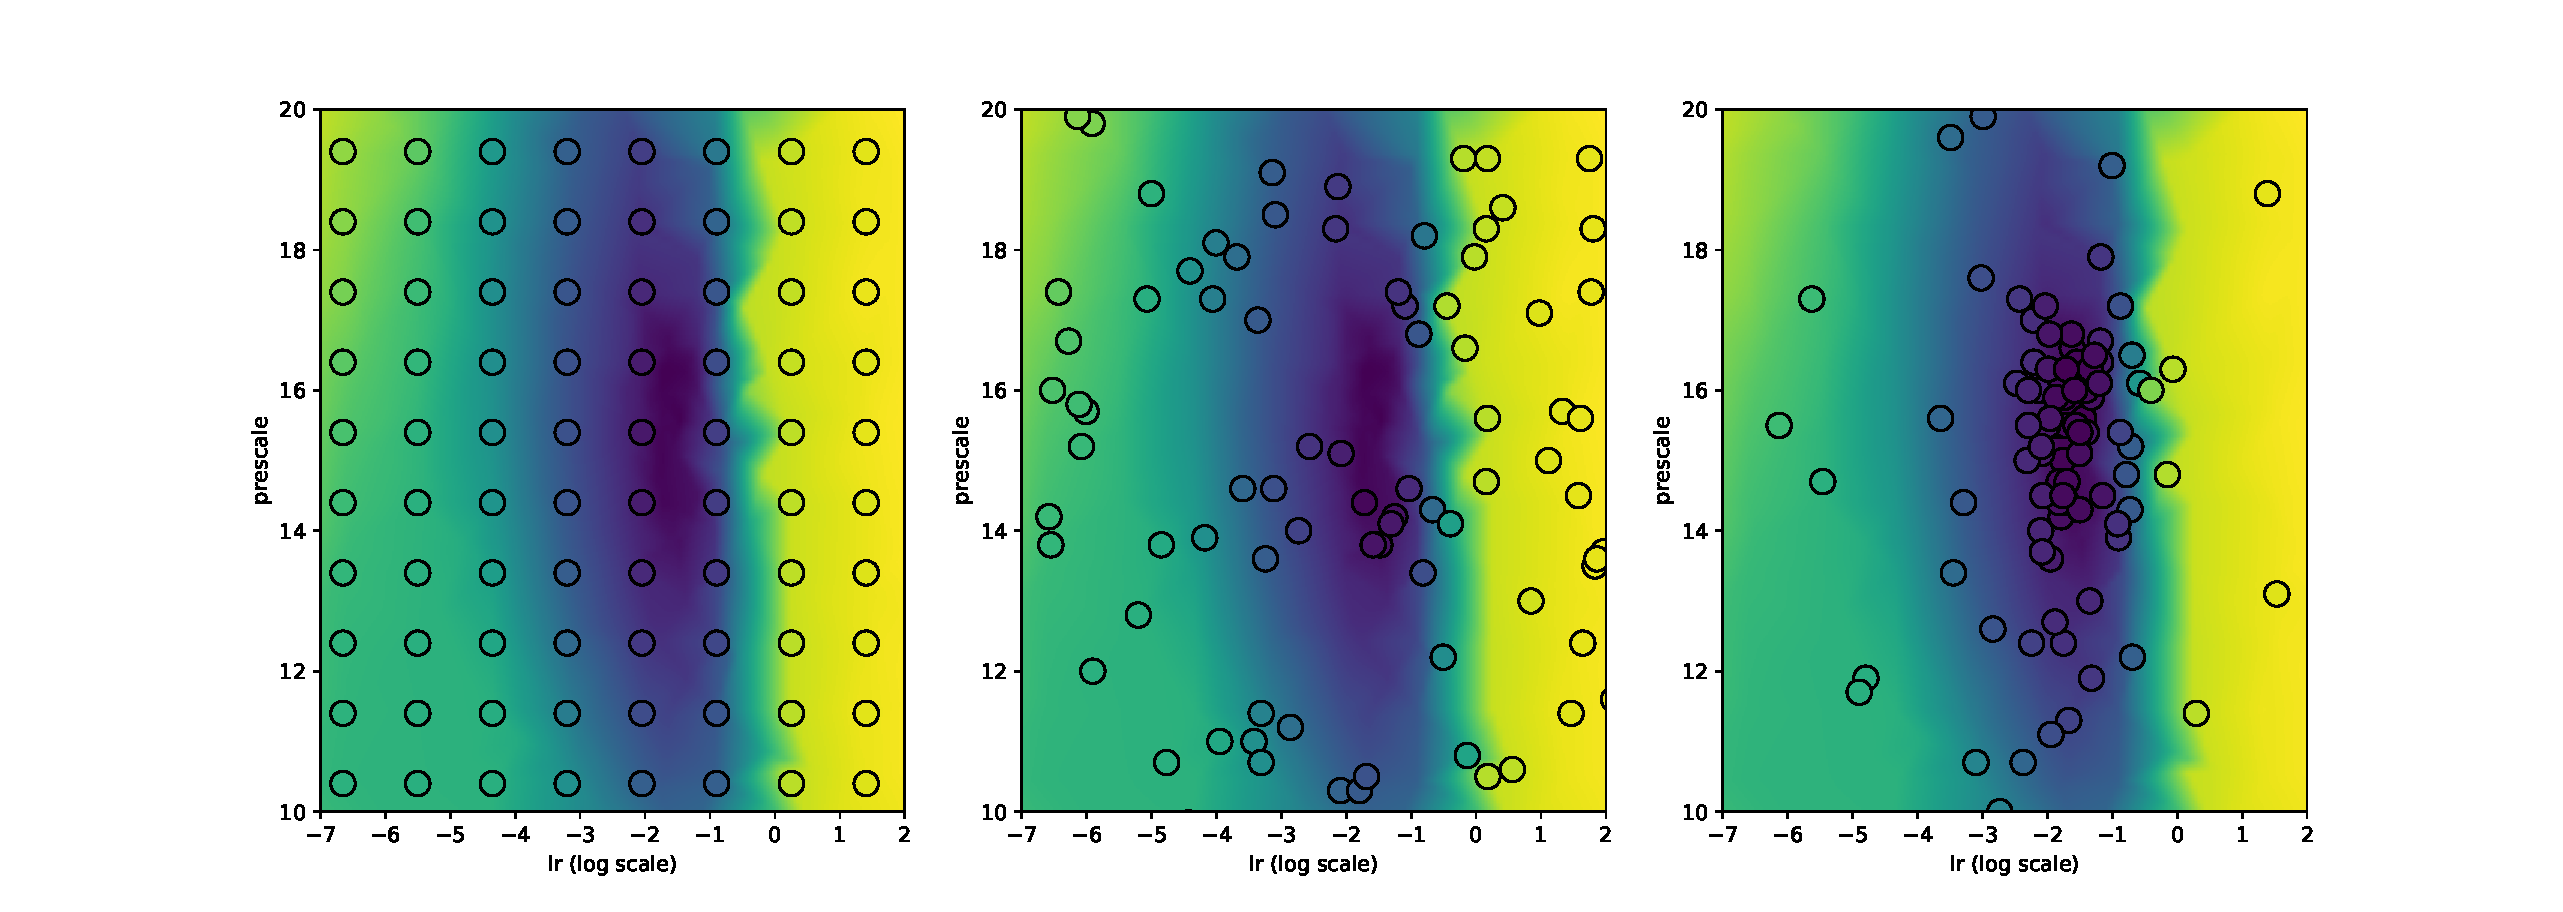
\includegraphics[width=1\textwidth]{figures/hp_search}\caption{Comparison of hyperparameter tuning methods. On the left a grid search,
in the middle a random search and on the right a biased random search.
Each experiment consisted in 100 iterations of SGD from a randomly
initialized network. We tune 2 hyperparameters on the x and y axis
(what they represent is not relevant here). The color scale represents
the final loss attained after a fixed number of iterations. The best
experiments are in blue, the worst experiments in yellow.}
\label{hptune-comparison}
\end{figure}


\section{A standard benchmark: Autoencoding written digits\label{sec:autoencoder-benchmark}}

We now describe the main benchmark that we will be using in the rest
of this document. The dataset MNIST \citep{lecun2010mnist} is composed
of 60.000 $28\times28$ grayscale images of handwritten digits, and
the corresponding value of the digit that is represented in the image.
For this benchmark, we use an autoencoder \ref{subsec:Autoencoders}
with layer sizes $\left\{ 784,1000,500,250,30,250,500,1000,784\right\} $.
The autoencoder encodes the input image into a vector of size $30$,
and then decodes it to reconstruct the original image. We use the
quadratic error $l\left(f\left(x\right),y\right)=\left\Vert f\left(x\right)-y\right\Vert _{2}^{2}$.
The benchmark consists in minimizing the empirical risk over the train
set after a fixed time on the same architecture.

This benchmark has a long history in the neural network optimization
litterature \citep{hinton2006reducing,martens2010deep,martens2015optimizing,desjardins2015natural}.
To assess the performance of an algorithm, we can use 2 metrics: the
empirical risk after a given number of iterations of the algorithm,
and the empirical risk after a fixed elapsed time for a given computer.
In real world tasks, the latter is more useful. It gives a better
understanding of the trade-off between a more complex update that
takes longer to compute and gives a better improvement, and a fast
update that gives a small improvement, but that can be iterated several
times in the meantime.

The limits of the benchmark are many. In particular the fact that
the state of the art papers in computer vision do not use MLPs and
sigmoid activations but rather variants of mixed convolutional networks
and residual connections, and variants of ReLU activations. Another
limit is in the use of the quadratic loss. Nonetheless, we still use
this benchmark as it is used by several other papers which allows
for a fair comparison, and because it is reasonably deep (8 layers)
and wide (the biggest weight matrix has size $1000\times784$).

\section{A classification task on an image dataset}

The second benchmark that we use is a multilayer perceptron with rectifier
activation functions, trained to recognize images amongst 10 classes
on the CIFAR-10 dataset \citep{torralba200880}. It is composed of
60.000 $32\times32$ color images, meaning that each image is composed
of $32*32*3=3072$ pixels. The network has 8 hidden layers of size
100 making it reasonably deep but still fast to train in order to
experiment with many algorithms. We train it using multiclass cross
entropy.

This architecture is far from producing state of the art results for
this task. In particular, it starts overfitting for a very small number
of updates. Instead, we use it to compare optimization algorithms,
which means that we are more interested in its performance on the
train set. If we were interested in generalization performance, we
could add regularization to better condition the optimization problem.

\chapter{Proof of concept: Evolution of the backpropagated gradient while
updating the parameters}

In this section, we present a prototype technique to account for the
interactions between parameters of different layers while computing
updates. While we could not come up with an efficient algorithm to
implement this technique, early results show that it could be useful
in deep networks.

\section{How is the gradient modified when changing the value of a parameter}

In usual gradient descent, we compute the gradient of the empirical
risk with respect to all parameters, then we update all parameters
at once. But since we are using backpropagation, then the process
of getting the partial derivatives is sequential, that is, we get
the derivatives of the top layers first, and afterwards we get the
derivatives of the bottom layers. Now suppose that we apply the update
for the parameters of the top layers before backpropagating through
it. The idea here is to estimate the new backpropagated signal. This
can also be interpreted as doing gradient descent separately for each
layer, but instead of recomputing the full forward and backward propagation
to the target layer, we just do a single updated backpropagation.

To illustrate the idea, we focus on the transformation computed by
a single layer:

\begin{eqnarray*}
h_{l} & = & f\left(a_{l}\right)\\
a_{l} & = & Wh_{l-1}+b
\end{eqnarray*}

Using backpropagation through this layer we get the partial derivative:

\begin{eqnarray}
\frac{\partial l}{\partial h_{l-1}} & = & \frac{\partial l}{\partial f}\frac{\partial f}{\partial a_{l}}\frac{\partial a_{l}}{\partial h_{l-1}}\nonumber \\
 & = & \frac{\partial l}{\partial f}\frac{\partial f}{\partial a_{l}}W\label{eq:dldhl}
\end{eqnarray}

This partial derivative is thus a function of $W$ in an explicit
way. It is also a function of $W$ and $b$ through the other terms
$\frac{\partial l}{\partial f}$ and $\frac{\partial f}{\partial a_{l}}$.
Can we get an update expression for $\frac{\partial l}{\partial h_{l-1}}\left(W+\Delta W,b+\Delta b\right)$?

\section{A first order update of a first order derivative}

A simple first order expansion gives a way of getting such an update:

\begin{align*}
\frac{\partial l}{\partial h_{l-1}}\left(W+\Delta W,b+\Delta b\right)\approx & \frac{\partial l}{\partial h_{l-1}}\left(W,b\right)+\frac{\partial}{\partial\text{vec}\left(W\right)}\left\{ \frac{\partial l}{\partial h_{l-1}}\left(W,b\right)\right\} \text{vec}\left(\Delta W\right)\\
 & +\frac{\partial}{\partial b}\left\{ \frac{\partial l}{\partial h_{l-1}}\left(W,b\right)\right\} \Delta b
\end{align*}

We used the vec operator in order to have a matrix expression for
the second derivative with respect to $W$. Using the expression \ref{eq:dldhl}
for $\frac{\partial l}{\partial h_{l-1}}$ we see that it requires
deriving 3 terms. Indeed the second derivative of the jacobian of
the input of the network, with respect to the preactivation $\frac{\partial f}{\partial a_{l}}$
is too costly to be used in a real problem. We choose not to use it.
The remaining 2 derivatives give an update:

\begin{eqnarray*}
\frac{\partial l}{\partial h_{l-1}}\left(W+\Delta W,b+\Delta b\right) & \approx & \left(\frac{\partial l}{\partial f}\frac{\partial f}{\partial a_{l}}\right)^{T}\Delta W+W^{T}\left(\frac{\partial f}{\partial a_{l}}\right)^{T}\frac{\partial^{2}l}{\partial f^{2}}\frac{\partial f}{\partial a_{l}}\left(\Delta Wh_{l-1}+\Delta b\right)
\end{eqnarray*}

In the process, we did 2 approximations: the first one in using a
first order expansion, the second one in not using the true second
derivatives, but instead just a part of them. We propose to replace
the backpropagation step by backpropagating this updated derivative.
We call this technique updated backpropagation (UBP), and we describe
a simple algorithm that implements it. Note that it requires backpropagating
a jacobian of the output of the network, in addition to the usual
gradient of the loss.

\begin{algorithm}[h]
\begin{algorithmic}[1]
\Require{$\mathcal{D}$ a minibatch of $n$ examples}
\Require{$\lambda$ learning rate}
\State{$dh_i \leftarrow \frac{\partial l}{\partial f_i}$}\Comment{Derivative of the loss w.r.t the output of the NN for each examples $i$}
\State{$J_i \leftarrow \sqrt{\frac{\partial^{2}l}{\partial f^{2}}}$}\Comment{Jacobian of the output of the NN for each examples $i$}
\ForAll{$l \in $ layers from top to bottom}
\State{$da_i \leftarrow dh_i \frac{\partial f_l^{(i)}}{\partial a_l^{(i)}}$}\Comment{Derivative of the loss w.r.t the preactivation for all examples $i$}
\State{$J_i \leftarrow J_i \frac{\partial f_l^{(i)}}{\partial a_l^{(i)}}$}
\State{$b\leftarrow b - \lambda \sum_i \left( da_i \right)^T$}\Comment{bias update}
\State{$W\leftarrow W - \lambda \sum_i da_i h_{l-1}^{(i)}$}\Comment{weights update}
\State{$dh_i \leftarrow da_i \left(W + \Delta W \right) + W^{T}J^T J \left(\Delta Wh_{l-1}^{(i)}+\Delta b\right)$}
\State{$J_i \leftarrow J_i W$}
\EndFor
\end{algorithmic}

\caption{Updated backpropagation}
\end{algorithm}


\section{Experiments}

We use the autoencoder benchmark to compare the performance of UBP
with stochastic gradient descent. Our results are plotted in figure
\ref{ubp-fig}. In terms of updates, we observe that this method outperforms
significantly compared to SGD (note that this is a logarithmic scale).
However it takes 10 times longer to obtain an update using UBP making
it unpractical on this task.

\begin{figure}
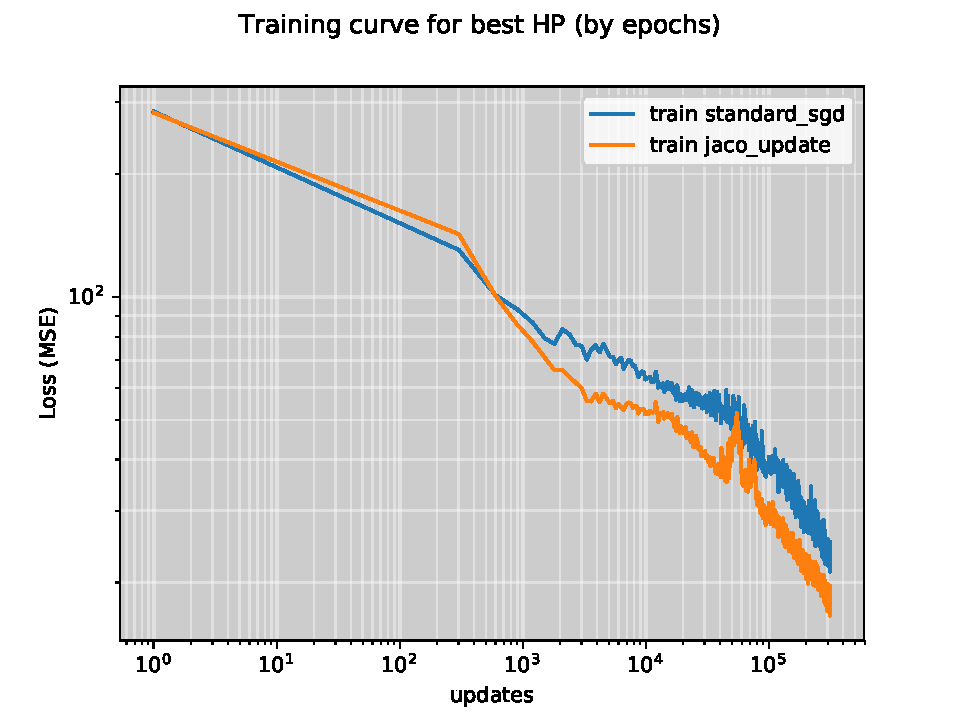
\includegraphics[width=0.7\textwidth]{figures/uab}\caption{Training error for standard backpropagation (in blue) and updated
backpropagation (in orange)}
\label{ubp-fig}
\end{figure}


\section{Limits of this method}

A first obvious limit is that it is very costly to compute the jacobians,
and also to store them in memory.

A second limit which can also be very problematic is that similarly
to the exploding gradient issue in deep or recurrent networks, we
observe that this update can cause the backpropagated gradients to
explode. Indeed, the problem resides in the fact that we have to multiply
by the square matrix $\left(\frac{\partial f}{\partial a_{l}}\right)^{T}\frac{\partial^{2}l}{\partial f^{2}}\frac{\partial f}{\partial a_{l}}$
at each layer. This matrix is a measure of how much will the preactivation
of the current layer change when we update its value by $\left(\Delta Wh+\Delta b\right)$.
But by use the chain rule, we can see that we will once again multiply
by this matrix when we compute the update of the next layer (which
is below as backpropagation computes the derivatives backward from
the top layer to the bottom layer). In the next layer, this matrix
will have the expression $\left(\frac{\partial f}{\partial a_{l-1}}\right)^{T}\frac{\partial^{2}l}{\partial f^{2}}\frac{\partial f}{\partial a_{l-1}}=\left(\frac{\partial a_{l}}{\partial a_{l-1}}\right)^{T}\left(\frac{\partial f}{\partial a_{l}}\right)^{T}\frac{\partial^{2}l}{\partial f^{2}}\frac{\partial f}{\partial a_{l}}\frac{\partial a_{l}}{\partial a_{l-1}}$,
so it will contain the former matrix. In this case, repeating this
process multiple times will do something like a power method, which
will either explode or vanish depending on the biggest eigenvalue
of $\left(\frac{\partial f}{\partial a_{l-1}}\right)^{T}\frac{\partial^{2}l}{\partial f^{2}}\frac{\partial f}{\partial a_{l-1}}$.

\section{Conclusion}

This current implementation is certainly not statisfying as a way
to accelerate optimization, because of its computational cost. Instead
we just see it as a proof of concept that it is possible to act on
the backpropagated signal in order to improve it. There are probably
more efficient ways of doing similar things, which could improve training
very deep networks, where it could account for the interactions between
layers that are separated by several others.

\chapter{Factorized second order\label{chap:Factorized-second-order}}

The expressions that we obtained for the FIM and the GN so far are
generic in the sense that they could be applied to any model and any
empirical risk composed of a sum of terms. We will now exploit the
very particular structure of neural networks, to obtain a better understanding
of how to apply these techniques for real tasks.

In an unconvenional way, we will start by presenting the local criterion
that we introduce, which allowed us to get competitive results, and
then we will introduce more general expressions and algorithms.

\section{A local criterion and the importance of the covariance of inputs
in a layer}

\subsection{Derivation of a new update\label{lol}}

Neural networks are usually trained using gradients computed all the
way from the loss function to the parameters. Inspired by target propagation
\citep{bengio2014auto,lee2015difference}, we explored an alternative
which consists in replacing the last step of the backpropagation algorithm:
the one of finding updates to the parameters given a derivative on
the preactivations. In figure \ref{fprop-bprop} (page \pageref{fprop-bprop})
we keep the usual computation for backpropagation (red lines) and
replace the part in green.

We now focus on a single layer $h_{l}=f_{l}\left(a_{l}\right)=f_{l}\left(W_{l}h_{l-1}+b_{l}\right)$
and from now on we will drop the subscript $l$ for brevity and write
$h'=f\left(a\right)=f\left(Wh+b\right)$. The gradients on the preactivation
are given by $\nabla_{a}l=\left(\frac{\partial l}{\partial a}\right)^{T}$
as usual. We formulate our local criterion as finding updates $\Delta W^{*},\Delta b^{*}$
so that in expectation we will match the opposite gradients of preactivations
times a learning rate $-\lambda\nabla_{a}l$. We call this optimization
problem ``local'' in the sense that it is formulated locally to
a single layer. We formulate our criterion as:

\begin{eqnarray*}
\Delta W^{*},\Delta b^{*} & = & \text{argmin}_{\Delta W,\Delta b}\frac{1}{n}\sum_{i}\left\Vert \Delta Wh^{(i)}+\Delta b+\lambda\nabla_{a^{(i)}}l\right\Vert _{2}^{2}+\epsilon\left\Vert \Delta W\right\Vert _{2}^{2}\\
 & = & \text{argmin}_{\Delta W,\Delta b}l_{C}\left(\Delta W,\Delta b\right)
\end{eqnarray*}

Instead of using gradient descent to find the optimal values for $\Delta W^{*},\Delta b^{*}$,
we directly solve this expression by taking derivatives with respect
to $\Delta W$ and $\Delta b$ and setting them to $0$:

\begin{eqnarray*}
\frac{\partial l_{C}}{\partial\Delta W} & = & \frac{1}{n}\sum_{i}\left(\Delta Wh^{(i)}+\Delta b+\lambda\nabla_{a^{(i)}}l\right)h^{(i)T}+\epsilon\Delta W\\
 & = & \Delta b\frac{1}{n}\sum_{i}h^{(i)T}+\epsilon\Delta W+\Delta W\frac{1}{n}\sum_{i}h^{(i)}h^{(i)T}+\frac{\lambda}{n}\sum_{i}\left(\nabla_{a^{(i)}}l\right)h^{(i)T}\\
\frac{\partial l_{C}}{\partial\Delta b} & = & \frac{1}{n}\sum_{i}\left(\Delta Wh^{(i)}+\Delta b+\lambda\nabla_{a^{(i)}}l\right)\\
 & = & \Delta b+\Delta W\frac{1}{n}\sum_{i}h^{(i)}+\frac{\lambda}{n}\sum_{i}\nabla_{a^{(i)}}l
\end{eqnarray*}

By putting both expressions together and simplifying for $\Delta W^{*}$
we get:

\begin{eqnarray*}
\Delta W^{*}\left(C+\epsilon\mathbf{I}\right) & = & -\frac{\lambda}{n}\sum_{i}\left(\nabla_{a^{(i)}}l\right)\left(h^{(i)}-\frac{1}{n}\sum_{i}h^{(i)}\right)^{T}\\
\Delta b^{*} & = & -\frac{\lambda}{n}\sum_{i}\nabla_{a^{(i)}}l-\frac{1}{n}\Delta W^{*}\sum_{i}h^{(i)}
\end{eqnarray*}

We denoted by $C=\frac{1}{n}\sum_{i}\left(h^{(i)}-\frac{1}{n}\sum_{i}h^{(i)}\right)\left(h^{(i)}-\frac{1}{n}\sum_{i}h^{(i)}\right)^{T}$
the covariance matrix of the activation of the previous layer. This
expressions can be solved by inverting the square matrix $\left(C+\epsilon\mathbf{I}\right)$.

\subsection{Comparison with standard SGD}

The updates for standard SGD are $\Delta_{SGD}b=-\frac{\lambda}{n}\sum_{i}\nabla_{a^{(i)}}l$
and $\Delta_{SGD}W=-\frac{\lambda}{n}\sum_{i}\left(\nabla_{a^{(i)}}l\right)h^{(i)T}$.

The \textbf{update for $b$} gets a new term $-\frac{1}{n}\Delta W\sum_{i}h^{(i)}$
that permits taking into account the update of $W$. In practice,
we found that it did not change much as $\Delta W$ is typically at
least one order of magnitude smaller than $\frac{\lambda}{n}\sum_{i}\nabla_{a^{(i)}}l$.

The \textbf{update for $W$ }is different in 2 ways. First, it is
also scaled using the inverse covariance matrix of the input $C^{-1}$.
Secondly, it is centered since we substract the expectation of $h$.
This is related to an old well used trick \citep{lecun1998gradient,schraudolph2012centering}.

\subsection{What is behind this local criteria}

This new update is somewhere between usual gradient descent, and something
that is inspired from target propagation. From a theoretical point
of view it is not yet clear why it would provide sensible updates.
Also surprising is the effectiveness of these new updates as we will
see in experimental section. In the following sections, we will show
that it is actually linked to second order methods applied to the
particular structure of neural networks.

\section{Decomposition using the Kronecker product\label{sec:Decomposition-using-the}}

In this section, we will show a convenient factorization of the Gauss-Newton
approximation of the Hessian, that was first applied to the Fisher
Information Matrix in the litterature \citep{martens2015optimizing}.
To this end, we will use an operation called the Kronecker product
that permits giving simple expressions for the GN matrix. For 2 matrices
$A$ of size $m\times n$ and $B$ of size $p\times q$ it produces
a new matrix $A\otimes B$ of size $mp\times nq$ defined by:

\begin{eqnarray*}
A\otimes B & = & \left(\begin{array}{ccc}
a_{11}B & \cdots & a_{1n}B\\
\vdots & \ddots & \vdots\\
a_{m1}B & \cdots & a_{mn}B
\end{array}\right)
\end{eqnarray*}

Its most interesting property in the context of neural networks is
its relationship with the $vec$ operation, that ``flattens'' a
matrix into a vector. It is of great use for 2nd order, because the
weight matrices can be vectorized using $vec$, to give matrix expressions
for the Hessian, which otherwise could not be written. We will make
use of the property:

\begin{eqnarray*}
vec\left(AXB\right) & = & \left(B^{T}\otimes A\right)vec\left(X\right)
\end{eqnarray*}

Getting back to the expression for the Gauss-Newton matrix derived
in section \ref{subsec:gauss-newton}, we use the block diagonal approximation
and focus on a single layer defined by the linear transformation $a=Wh+b$
and the nonlinearity $h'=f\left(a\right)$. We start from the jacobian
of the output of the network, with respect to the output of the linear
transformation $a$, denoted by $\mathbf{J}_{a}$. From this jacobian
computed by backpropagation, we can get the jacobian with respect
to the parameters of the layer by making use of the chain rule $\mathbf{J}_{\theta}=\mathbf{J}_{a}\mathbf{J}_{\theta}^{a}$.
We use the notation $\mathbf{J}_{\theta}^{a}$ for the jacobian of
$a$ with respect to $\theta$. In order to get an expression for
this jacobian, we now make use of the $vec$ operator to transform
$W$ into a vector:

\begin{eqnarray*}
a & = & vec\left(a\right)\\
 & = & vec\left(Wh\right)+b\\
 & = & \left(h^{T}\otimes\mathbf{I}\right)vec\left(W\right)+b
\end{eqnarray*}

$\mathbf{I}$ is the identity, of the same size as $a$, that is the
output size of the layer. We can now give an expression for $\mathbf{J}_{vec\left(W\right)}^{a}$
and $\mathbf{J}_{b}^{a}$:

\begin{eqnarray*}
\mathbf{J}_{b}^{a} & = & \mathbf{I}\\
\mathbf{J}_{vec\left(W\right)}^{a} & = & h^{T}\otimes\mathbf{I}
\end{eqnarray*}

Or, if we stack $vec\left(W\right)$ and $b$ in a vector $\theta$:

\begin{eqnarray*}
\mathbf{J}_{\theta}^{a} & = & \left(\begin{array}{cc}
h^{T} & 1\end{array}\right)\otimes\mathbf{I}
\end{eqnarray*}

And finally by the chain rule:

\begin{eqnarray}
\mathbf{J}_{\theta} & = & \left(\begin{array}{cc}
h^{T} & 1\end{array}\right)\otimes\mathbf{J}_{a}\label{eq:jaco_factorization}
\end{eqnarray}

where $\left(\begin{array}{cc}
h^{T} & 1\end{array}\right)$ is the concatenation of the row vector $h^{T}$ and $1$.

This jacobian is a first order measure of how much the output of the
network will change if we change the values of the parameters of this
layer, for a single example. Let us now recall the expression of the
GN matrix $G_{f}=\frac{1}{n}\sum_{i}\mathbf{J}_{\theta}\left(x_{i}\right)^{T}D\left(x_{i}\right)\mathbf{J}_{\theta}\left(x_{i}\right)$
from section \ref{subsec:gauss-newton}. We can rewrite this expression
using the factorization in eq \ref{eq:jaco_factorization}:
\begin{eqnarray}
G_{f} & = & \frac{1}{n}\sum_{i}\left[\left(\begin{array}{cc}
h_{i}^{T} & 1\end{array}\right)\otimes\mathbf{J}_{a_{i}}\right]^{T}D\left(x_{i}\right)\left[\left(\begin{array}{cc}
h_{i}^{T} & 1\end{array}\right)\otimes\mathbf{J}_{a_{i}}\right]\nonumber \\
 & = & \frac{1}{n}\sum_{i}\left(\begin{array}{cc}
h_{i}^{T} & 1\end{array}\right)^{T}\left(\begin{array}{cc}
h_{i}^{T} & 1\end{array}\right)\otimes\left(\mathbf{J}_{a_{i}}^{T}D\left(x_{i}\right)\mathbf{J}_{a_{i}}\right)\nonumber \\
 & = & \frac{1}{n}\sum_{i}\left(\begin{array}{cc}
h_{i}h_{i}^{T} & h_{i}\\
h_{i}^{T} & 1
\end{array}\right)\otimes\left(\mathbf{J}_{a_{i}}^{T}D\left(x_{i}\right)\mathbf{J}_{a_{i}}\right)\label{eq:factored}
\end{eqnarray}

We used the property that $\left(A\otimes B\right)\left(C\otimes D\right)=AC\otimes BD$
when the sizes of the matrices $A,B,C,D$ match. This factorization
is interesting because it separates the GN matrix into a contribution
from the backpropagated jacobian (red arrow in figure \ref{fprop-bprop}
page \pageref{fprop-bprop}), and a part that only uses the forward
statistics and that is local to a layer. While these 2 contributions
are clearly factorized for a single example, it is not clear whether
the resulting sum can still be factorized using a kronecker product.
As we will show in the next section, similar factorizations were exploited
in KFAC \citep{martens2015optimizing} and Natural Neural Networks
\citep{desjardins2015natural} to build efficient optimization algorithms.
Note that in this formulation in eq \ref{eq:factored} we contribute
an explicit distinction between the weight matrix $W$ and the bias
$b$ whereas in previous work authors usually put all parameters together
in a weight matrix with an extra column. As we will see in future
sections, this is key to understanding the role of centering the updates.

\subsection{Decomposition into 2 smaller matrices}

In second order algorithms, inverting the Hessian matrix is often
the limiting factor as its computational cost is $O\left(n^{3}\right)$.
The Kronecker product as the pleasing property that it turns the inversion
of a big matrix into inverting 2 smaller matrices since $\left(A\otimes B\right)^{-1}=A^{-1}\otimes B^{-1}$.
In our case, if such a decomposition existed we would reduce the computational
cost from $O\left(n_{in}^{3}n_{out}^{3}\right)$ to $O\left(n_{in}^{3}\right)+O\left(n_{out}^{3}\right)$.

Unfortunately, we can not write the GN matrix nor the FIM using 2
matrices because it is a sum of Kronecker products, so we aim at finding
approximate factorizations that will have the required form.

\subsection{Focus on the covariance part of the decomposition\label{subsec:focus-covariance}}

We now suppose that we can use the following approximation:

\begin{eqnarray}
\frac{1}{n}\sum_{i}\left(\begin{array}{cc}
h_{i}h_{i}^{T} & h_{i}\\
h_{i}^{T} & 1
\end{array}\right)\otimes\left(\mathbf{J}_{a_{i}}^{T}D\left(x_{i}\right)\mathbf{J}_{a_{i}}\right) & \approx & \frac{1}{n}\sum_{i}\left(\begin{array}{cc}
h_{i}h_{i}^{T} & h_{i}\\
h_{i}^{T} & 1
\end{array}\right)\otimes\alpha\mathbf{I}=G_{in}\label{eq:approx_alpha}
\end{eqnarray}

Here $\alpha$ does not depend on $i$. This approximation means that
we ignore the interactions between the output preactivations. Instead
we just focus on some statistics of the activations of the current
layer. Looking back at the use we will make of this preconditioner,
we can interpret it as penalizing an update if the corresponding activation
has a high variance. This makes sense since in this case changing
the value here will change the next forward propagated signal more
that if the variance of the corresponding activation were lower. This
would result in a bigger expected change in the output. 

The left part $A=\frac{1}{n}\sum_{i}\left(\begin{array}{cc}
h_{i}h_{i}^{T} & h_{i}\\
h_{i}^{T} & 1
\end{array}\right)$ corresponds to some statistics on the input of the considered layer.
It has the size $\left(n_{in}+1\right)\times\left(n_{in}+1\right)$
with the line/column corresponding to the bias. We will now derive
the update that corresponds to using this matrix $G_{in}$ as a preconditioner:

We need to invert $A$. This matrix can be inverted blockwise. We
denote by $C=\frac{1}{n}\sum_{i}\left(h_{i}-\frac{1}{n}\sum_{j}h_{j}\right)\left(h_{i}-\frac{1}{n}\sum_{j}h_{j}\right)^{T}$the
covariance matrix of the input vector of the linear layer. We get
the inverse:

\begin{eqnarray*}
\left(\begin{array}{cc}
\frac{1}{n}\sum_{i}h_{i}h_{i}^{T} & \frac{1}{n}\sum_{i}h_{i}\\
\frac{1}{n}\sum_{i}h_{i}^{T} & 1
\end{array}\right)^{-1} & = & \left(\begin{array}{cc}
C^{-1} & -C^{-1}\frac{1}{n}\sum_{i}h_{i}\\
-\frac{1}{n}\sum_{i}h_{i}^{T}C^{-1} & 1+\frac{1}{n}\sum_{i}h_{i}^{T}C^{-1}\frac{1}{n}\sum_{i}h_{i}
\end{array}\right)
\end{eqnarray*}

Applying this preconditioner to a gradient update we can get a new
update for the weight matrix and the bias. Let us first recall the
gradient for a minibatch of examples. In order to be able to use it
with our preconditioner we put the parameters into a vector $\theta=\left(\begin{array}{cc}
\text{vec}\left(W\right)^{T} & b^{T}\end{array}\right)^{T}$:

\begin{eqnarray*}
\nabla_{\theta}R & = & -\frac{\lambda}{n}\sum_{j}\left(\begin{array}{c}
h_{j}\\
1
\end{array}\right)\otimes\nabla_{a_{j}}l
\end{eqnarray*}

The corresponding update is a Newton step using the approximate Hessian
(see eq \ref{eq:newton-step} page \pageref{eq:newton-step}):

\begin{eqnarray*}
G_{in}^{-1}\nabla_{\theta}R & = & \frac{1}{n}\sum_{j}\left(\begin{array}{cc}
C^{-1} & -C^{-1}\frac{1}{n}\sum_{i}h_{i}\\
-\frac{1}{n}\sum_{i}h_{i}^{T}C^{-1} & 1+\frac{1}{n}\sum_{i}h_{i}^{T}C^{-1}\frac{1}{n}\sum_{i}h_{i}
\end{array}\right)\left(\begin{array}{c}
h_{j}\\
1
\end{array}\right)\otimes\frac{-\lambda}{\alpha}\nabla_{a_{j}}l
\end{eqnarray*}

From this expression we can write the update for $W$:

\begin{eqnarray*}
\Delta\text{vec}\left(W\right) & = & C^{-1}\frac{-\lambda}{n}\sum_{j}h_{j}\otimes\frac{1}{\alpha}\nabla_{a_{j}}l-C^{-1}\frac{1}{n}\sum_{i}h_{i}\otimes\frac{-\lambda}{n}\sum_{j}\frac{1}{\alpha}\nabla_{a_{j}}l\\
 & = & \frac{1}{\alpha}C^{-1}\frac{-\lambda}{n}\sum_{j}\left(h_{j}-\frac{1}{n}\sum_{i}h_{i}\right)\otimes\nabla_{a_{j}}l
\end{eqnarray*}
\begin{equation}
\boxed{\Delta W=\frac{-\lambda}{\alpha}\frac{1}{n}\sum_{j}\nabla_{a_{j}}l\left(h_{j}-\frac{1}{n}\sum_{i}h_{i}\right)^{T}C^{-1}}\label{eq:upd_w}
\end{equation}

And the update for $b$:

\begin{eqnarray*}
\Delta b & = & -\frac{-\lambda}{n}\sum_{j}\frac{1}{n}\sum_{i}h_{i}^{T}C^{-1}h_{j}\frac{1}{\alpha}\nabla_{a_{j}}l+\left(1+\frac{1}{n}\sum_{i}h_{i}^{T}C^{-1}\frac{1}{n}\sum_{i}h_{i}\right)\frac{-\lambda}{n}\sum_{j}\frac{1}{\alpha}\nabla_{a_{j}}l\\
 & = & \frac{-\lambda}{n}\sum_{j}\frac{1}{\alpha}\nabla_{a_{j}}l+\frac{\lambda}{n}\sum_{j}\frac{1}{n}\sum_{i}h_{i}^{T}C^{-1}\left(h_{j}-\frac{1}{n}\sum_{i}h_{i}\right)\frac{1}{\alpha}\nabla_{a_{j}}l
\end{eqnarray*}
\begin{equation}
\boxed{\Delta b=-\frac{\lambda}{\alpha}\frac{1}{n}\sum_{j}\nabla_{a_{j}}l-\Delta W\frac{1}{n}\sum_{i}h_{i}}\label{eq:upd_b}
\end{equation}

Using an argument based on second order methods, we thus get back
to the very same update as in eq \ref{lol}.

\section{Algorithms}

We now present 2 algorithms. The first one is very simple and just
aims at isolating the centering trick, in order to assess how much
of the gain of performance comes from just centering the update, and
how much comes from the whole covariance. The other one is the full
update that we just derived.

\subsection{Centered gradient descent\label{subsec:Centered-gradient-descent}}

Following the update for $W$ derived in eq \ref{eq:upd_w}, we simply
replace the usual update for the weight matrices by a centered version
$\Delta W=\frac{1}{n}\sum_{j}\nabla_{a_{j}}l\left(h_{j}-\overbrace{\frac{1}{n}\sum_{i}h_{i}}^{\text{centering}}\right)^{T}$.
The gradient, as well as the inner expectation, are computed using
a minibatch. Some author refer to a very similar idea as \textit{mean-only
batch normalization} \citep{salimans2016weight} where the value of
$h$ is replaced by $h-\mathbb{E}\left[h\right]$ in the forward pass,
with the expectation being computed using a mini-batch. The difference
here is that we do not reparametrize the forward propagation, instead
we just follow a slightly different direction which is not the gradient
but a centered gradient, as suggested by eq \ref{eq:upd_w}.

\begin{algorithm}
\begin{algorithmic}[1]
\While{not converged}
\State{Sample a minibatch $\mathcal{D}$}
\For{all layers}
\State{$\Delta_{a_i}\leftarrow\nabla_{a_i} l\left(f\left(x_i\right), y_i\right) \forall i \in \mathcal{D}$}
\State{$b\leftarrow b + \lambda \frac{1}{n} \sum_i \Delta_{a_i}$}
\State{$W\leftarrow W + \lambda \frac{1}{n} \sum_i \Delta_{a_i} \left(h_{i}-\frac{1}{n}\sum_{j}h_{j}\right)^T $}
\EndFor
\EndWhile
\end{algorithmic}

\caption{Centered gradient descent}

\end{algorithm}


\subsection{Amortized covariance preconditioner\label{subsec:Amortized-covariance-preconditio}}

In the updates derived from the covariance (for $b$ eq \ref{eq:upd_b}
and for $W$ eq \ref{eq:upd_w}), we require an inverse of the matrix
$C=\frac{1}{n}\sum_{i}\left(h_{i}-\frac{1}{n}\sum_{j}h_{j}\right)\left(h_{i}-\frac{1}{n}\sum_{j}h_{j}\right)^{T}$.
This matrix has the size of the input of a layer $n_{in}$. While
it is smaller than the full GN or FIM for a single layer of size $\left(n_{in}+1\right)\times n_{out}$,
it is still not very efficient to estimate the inverse at each iteration.
Meanwhile, these statistics do not change much between iterations
so a natural idea is to amortize the cost of inversion over several
updates.

A question remains for the choice of $\alpha$ that we used to approximate
the real GN matrix in eq \ref{eq:approx_alpha}. We adopt two approaches.
The first one consists in treating it as a fixed value, so it is a
hyperparameter that we tune using our biased random search (section
\ref{biased-random-search}). The second one is a very experimental
heuristic, which consists in taking the maximum value of the squarred
gradient $\alpha=\max_{i\in\text{minibatch},j\leq n_{out}}\left(\nabla_{a_{i}}l\right)_{j}^{2}$.
This gives a different value for each layer, and also different for
each minibatch. We found it worked very well experimentally, and we
justify it as being a rough heuristic estimate of the curvature of
the empirical risk, with respect to the output of the layer.

For numerical stability and to account for the imprecision of $C$
between two estimates, we use Tikhonov regularization (section \ref{tikhonov}).
This adds a scalar value $\epsilon$ to the diagonal of our approximate
GN, which in this case is scaled by $\frac{1}{\alpha}$:

\begin{eqnarray*}
\frac{1}{n}\sum_{i}\left(\begin{array}{cc}
h_{i}h_{i}^{T} & h_{i}\\
h_{i}^{T} & 1
\end{array}\right)\otimes\alpha\mathbf{I}_{out}+\epsilon\mathbf{I} & = & \frac{1}{n}\sum_{i}\left(\begin{array}{cc}
h_{i}h_{i}^{T}+\frac{\epsilon}{\alpha}\mathbf{I} & h_{i}\\
h_{i}^{T} & 1+\frac{\epsilon}{\alpha}
\end{array}\right)\otimes\alpha\mathbf{I}_{out}
\end{eqnarray*}

and the updated covariance matrix becomes:

\begin{eqnarray*}
C & = & \frac{1}{n}\sum_{i}\left(h_{i}-\frac{1}{n}\sum_{j}h_{j}\right)\left(h_{i}-\frac{1}{n}\sum_{j}h_{j}\right)^{T}+\frac{\epsilon}{\alpha}\mathbf{I}
\end{eqnarray*}

\begin{algorithm}
\begin{algorithmic}[1]
\Require{$\mathbf{N}$  estimate statistics every $\mathbf{N}$ minibatches}
\State{$n_{updates} \leftarrow 0$}
\While{not converged}
\If{$n_{updates}\mod\mathbf{N}=0$}
\State{Sample a minibatch $\mathcal{D}$}
\For{each layer $j$}
\State{$C^{\left(j\right)} \leftarrow \text{cov} \left(h^{\left(j\right)}, h^{\left(j\right)} \right)$}
\State{$inv\_C^{\left(j\right)} \leftarrow \text{inverse} \left( C^{\left(j\right)}+\frac{\epsilon}{\alpha}\mathbf{I} \right)$}

\EndFor
\EndIf
\State{Sample a minibatch $\mathcal{D}$}
\For{each layer $j$}
\State{$\Delta_{a_i^{\left(j\right)}}\leftarrow\nabla_{a_i^{\left(j\right)}} l\left(f\left(x_i\right), y_i\right) \forall i \in \mathcal{D}$}
\State{$b\leftarrow b + \frac{\lambda}{\alpha} \frac{1}{n} \sum_i \Delta_{a_i^{\left(j\right)}}$}
\Comment{eq \ref{eq:upd_b}}
\State{$W\leftarrow W + \frac{\lambda}{\alpha} \frac{1}{n} \sum_i \Delta_{a_i^{\left(j\right)}} \left(h_{i}^{\left(j\right)}-\frac{1}{n}\sum_{k}h_{k}^{\left(j\right)}\right)^T inv\_C^{\left(j\right)}$}
\Comment{eq \ref{eq:upd_w}}
\EndFor
\State{$n_{updates} \leftarrow n_{updates} + 1$}
\EndWhile
\end{algorithmic}

\caption{Amortized covariance preconditioner (ACP)}
\end{algorithm}


\section{Other related approximate second order algorithms}

The 2 following techniques have been proposed using the same factorization
of the FIM that we wrote in eq \ref{eq:factored}. In addition to
their factorization we introduced the explicit separation of weight
matrix and bias, which we use in the following notations.

\subsection{KFAC}

KFAC \citep{martens2015optimizing} proposed to split the sum of Kronecker
products into a product of sums:
\begin{eqnarray*}
\mathbf{F} & \approx & \mathbb{E}\left[\left(\begin{array}{cc}
hh^{T} & h\\
h^{T} & 1
\end{array}\right)\right]\otimes\mathbb{E}\left[\left(\boldsymbol{J}_{\boldsymbol{y}}^{a}\right)^{T}D\left(\boldsymbol{y}\right)\boldsymbol{J}_{\boldsymbol{y}}^{a}\right]
\end{eqnarray*}

The Kronecker product has the nice property that for 2 invertible
square matrices $A$ and $B$, $\left(A\otimes B\right)^{-1}=A^{-1}\otimes B^{-1}$.
It follows that inverting the FIM now requires inverting 2 smaller
matrices. As for the approximation we made in eq \ref{eq:approx_alpha}
section \ref{subsec:focus-covariance}, we lose the coupling between
both parts of the kronecker product of each example in the FIM (see
eq \ref{eq:factored} page \pageref{eq:factored}). In our experiments
we found a comparable performance between KFAC and ACP.

KFAC has been introduced for the natural gradient, but as we shown
in the previous sections, it can also be adapted to Gauss-Newton.

\subsection{Natural Neural Networks}

Natural neural networks \citep{desjardins2015natural} exploit the
same factorization by focusing on the input covariance part of each
layer. They propose a reparametrization that makes $\mathbb{E}\left[hh^{T}\right]$
equal the identity. They also notice that in order for their method
to work well, they have to use the centering trick. To this view,
they change the original linear transformation $a=Wh+b$ to become:

\begin{eqnarray*}
a & = & VU\left(h-\mu\right)+d
\end{eqnarray*}

$V$ is the new weight matrix and $d$ are the new biases. $\mu=\mathbb{E}\left[h\right]$
is the mean value for $h$ and $U$ is the square root of the inverse
covariance of $h$, defined by $U^{2}=\left(\mathbb{E}\left[\left(h-\mu\right)\left(h-\mu\right)^{T}\right]\right)^{-1}$,
denoted by $U=\left(\mathbb{E}\left[\left(h-\mu\right)\left(h-\mu\right)^{T}\right]\right)^{-\frac{1}{2}}$.
$U$ and $\mu$ are not trained using gradient descent but instead
they are estimated using data from the training set.

The new parameters $V$ and $d$ are trained using gradient descent.
We will denote by $h_{e}=U\left(h-\mu\right)$ the new ``effective''
input to the linear transformation induced by the weight matrix $V$.
Let us first remark that $\mathbb{E}\left[h_{e}\right]=U\left(\mathbb{E}\left[h\right]-\mu\right)=U\left(\mu-\mu\right)=0$,
so the reparametrized input is centered on average. A second remark
is that $\mathbb{E}\left[h_{e}h_{e}^{T}\right]=U\mathbb{E}\left[\left(h-\mu\right)\left(h-\mu\right)^{T}\right]U^{T}=\mathbf{I}$.
By construction $U$ cancels out the covariance. Wrapping everything
together we thus have the desired property that:

\begin{eqnarray*}
\mathbb{E}\left[\left(\begin{array}{cc}
h_{e}h_{e}^{T} & h_{e}\\
h_{e}^{T} & 1
\end{array}\right)\right] & = & \left(\begin{array}{cc}
\mathbb{E}\left[h_{e}h_{e}^{T}\right] & \mathbb{E}\left[h_{e}\right]\\
\mathbb{E}\left[h_{e}^{T}\right] & 1
\end{array}\right)\\
 & = & \left(\begin{array}{cc}
\mathbf{I} & 0\\
0 & 1
\end{array}\right)
\end{eqnarray*}

The approximate FIM for the reparametrization thus has a better form.
In this case the natural gradient update will be closer to the usual
gradient update.

\section{Experiments}

\subsection{Centering tricks}

We compare our algorithms using the autoencoder benchmark presented
in section \ref{sec:autoencoder-benchmark}. We ran all experiments
on the same architecture using a Titan Black GPU.

For each experiment we plot the expected loss on the train set, and
on a test set that we did not use for learning (figure \ref{centering}).
To assess the practical performance, the x-axis represents the actual
time spent on each experiment. We selected the best hyperparameters
using biased random search, and we only plot the best experiment.
For the test experiments, we also only plot the best result for each
technique. We ran each experiment for $3\times10^{5}$ updates.

\begin{figure}[h]
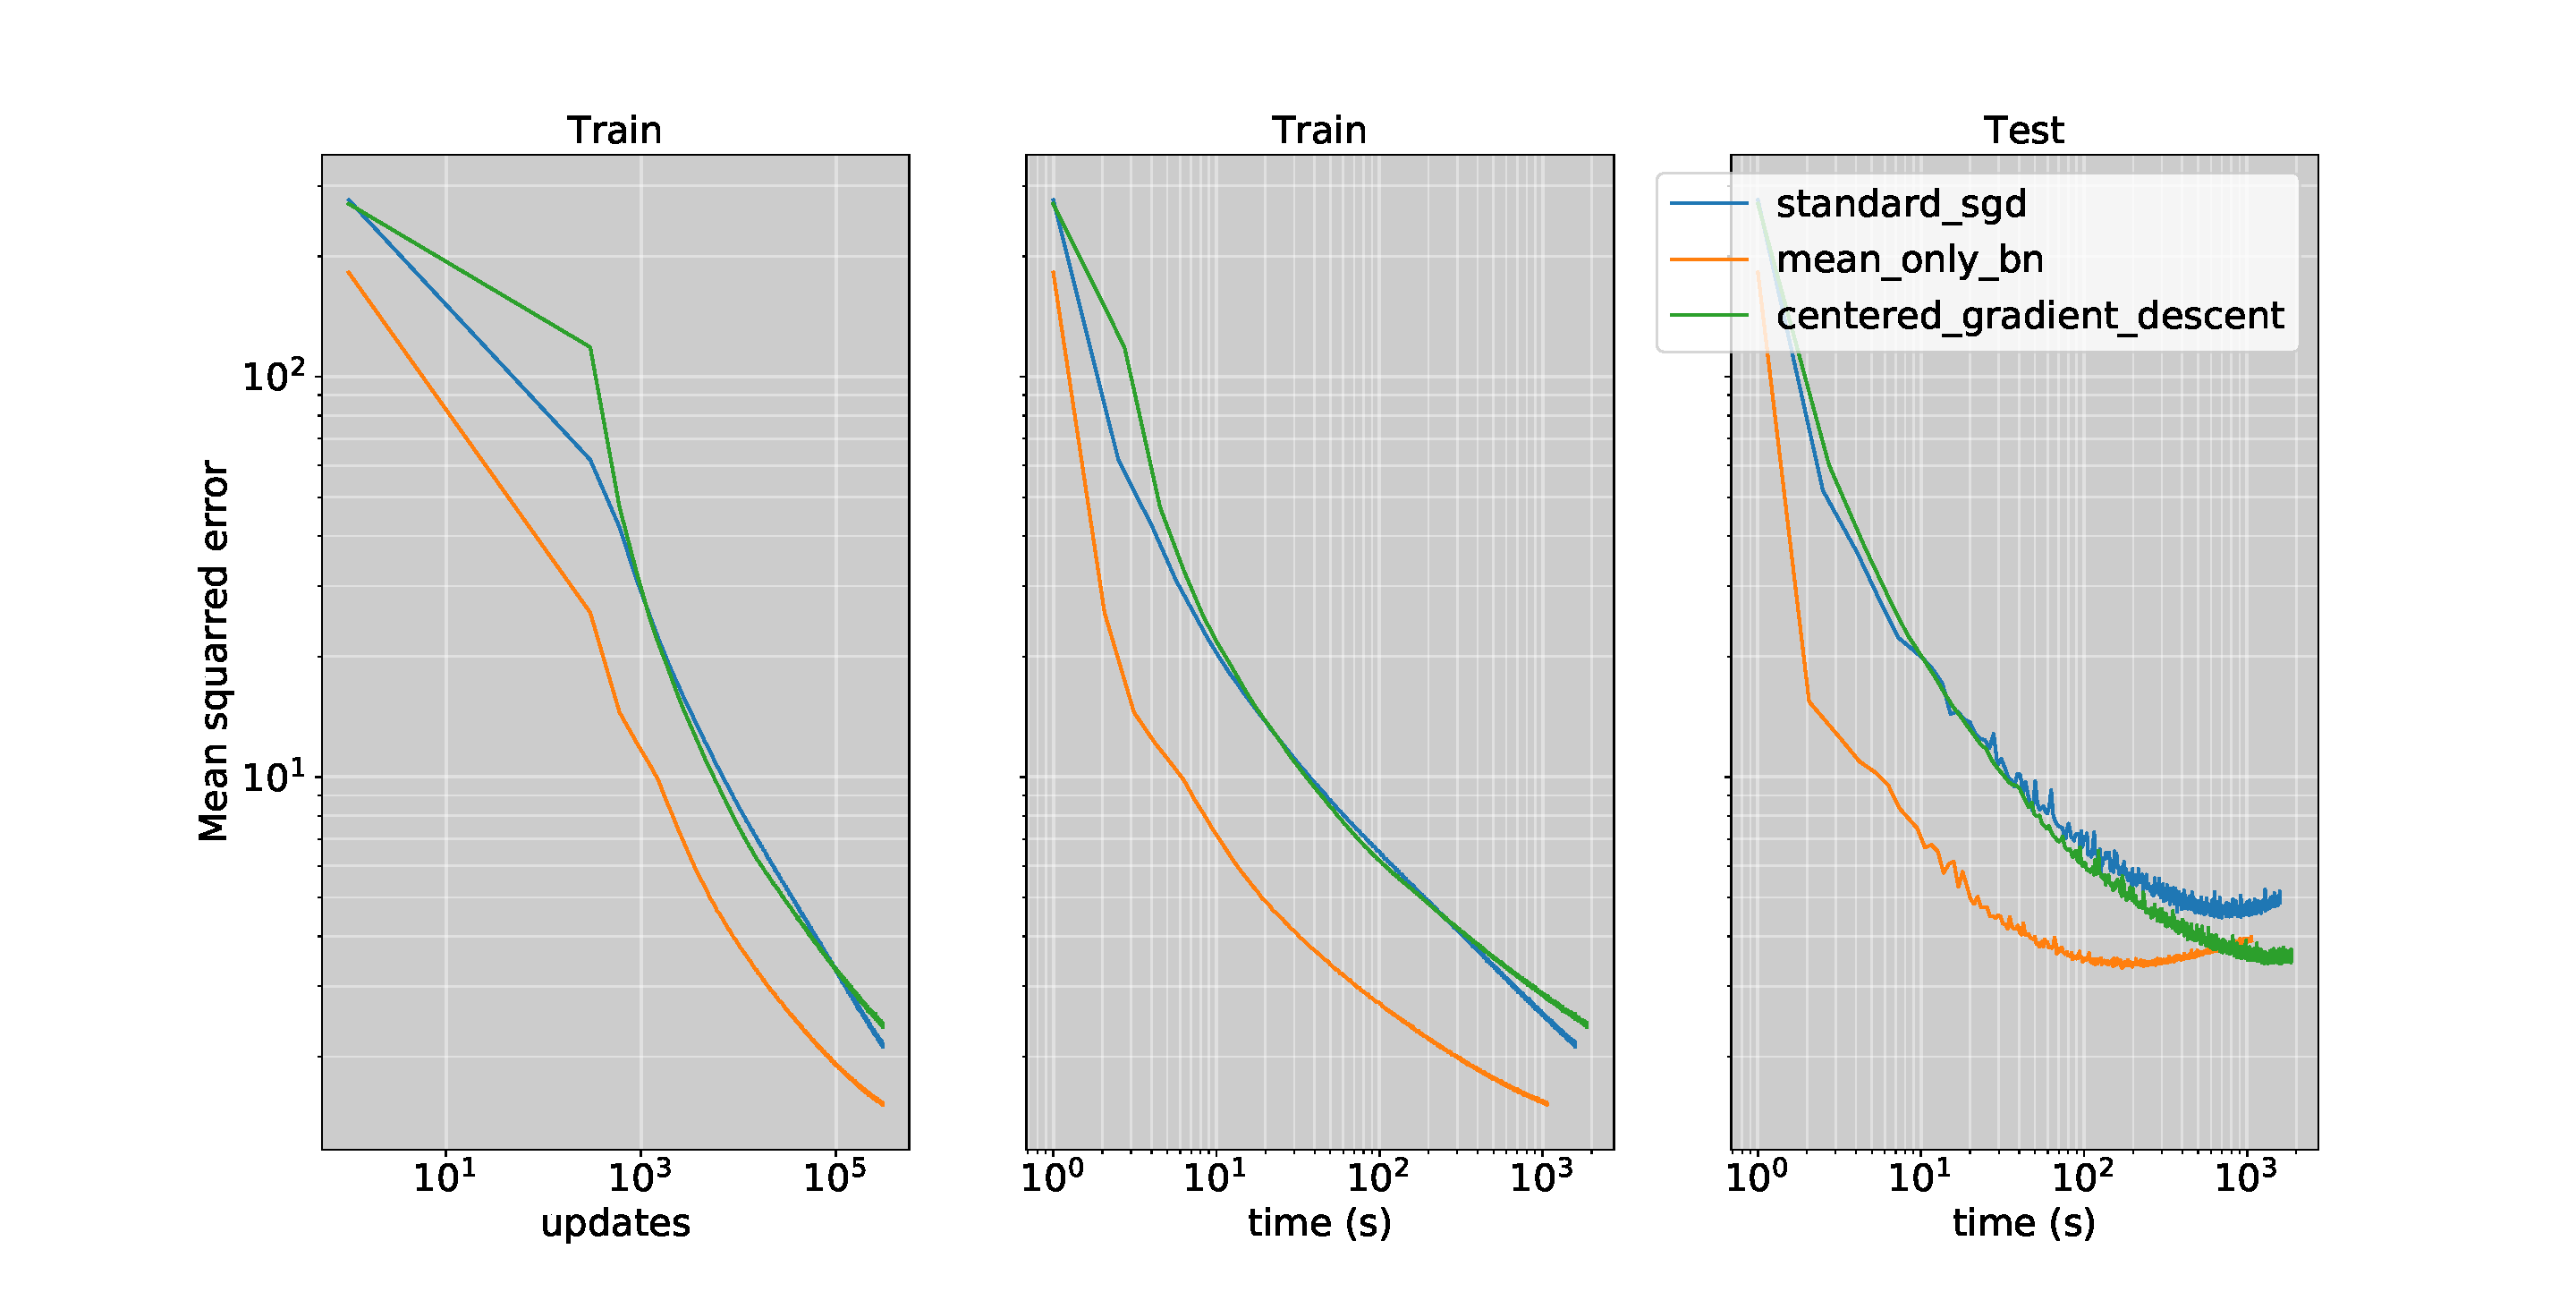
\includegraphics[width=1\textwidth]{figures/centering}

\caption{Comparison of centering methods on MNIST autoencoder: blue: standard
SGD with fixed learning rate; orange: mean-only batch norm; green:
centered updates as presented in section \ref{subsec:Centered-gradient-descent};
red: ACP with fixed $\alpha$ as presented in section \ref{subsec:Amortized-covariance-preconditio}.}
\label{centering}

\end{figure}


\subsection{Comparison of 2nd order approximate methods}

In the second experiment, we compare all second order approximations
to a baseline using batch normalization on the autoencoder on MNIST.
For all experiments we use an amortization factor of 100, that is
we update the statistics and invert the corresponding matrices every
100 updates. We use a minibatch size of 200 for each update as well
as for the statistics. See figure \ref{mnist-autoencoder}.

In a third experiment, we compare all second order approximate methods
on the classification task on CIFAR10. Similarly to the autoencoder,
we use a minibatch size of 200, and we recompute the inverse statistics
every 100 updates. As all methods are able to overfit very rapidly,
we also report the error rate on both the train set and a separated
test set. See figure \ref{cifar10}.

\begin{figure}[h]
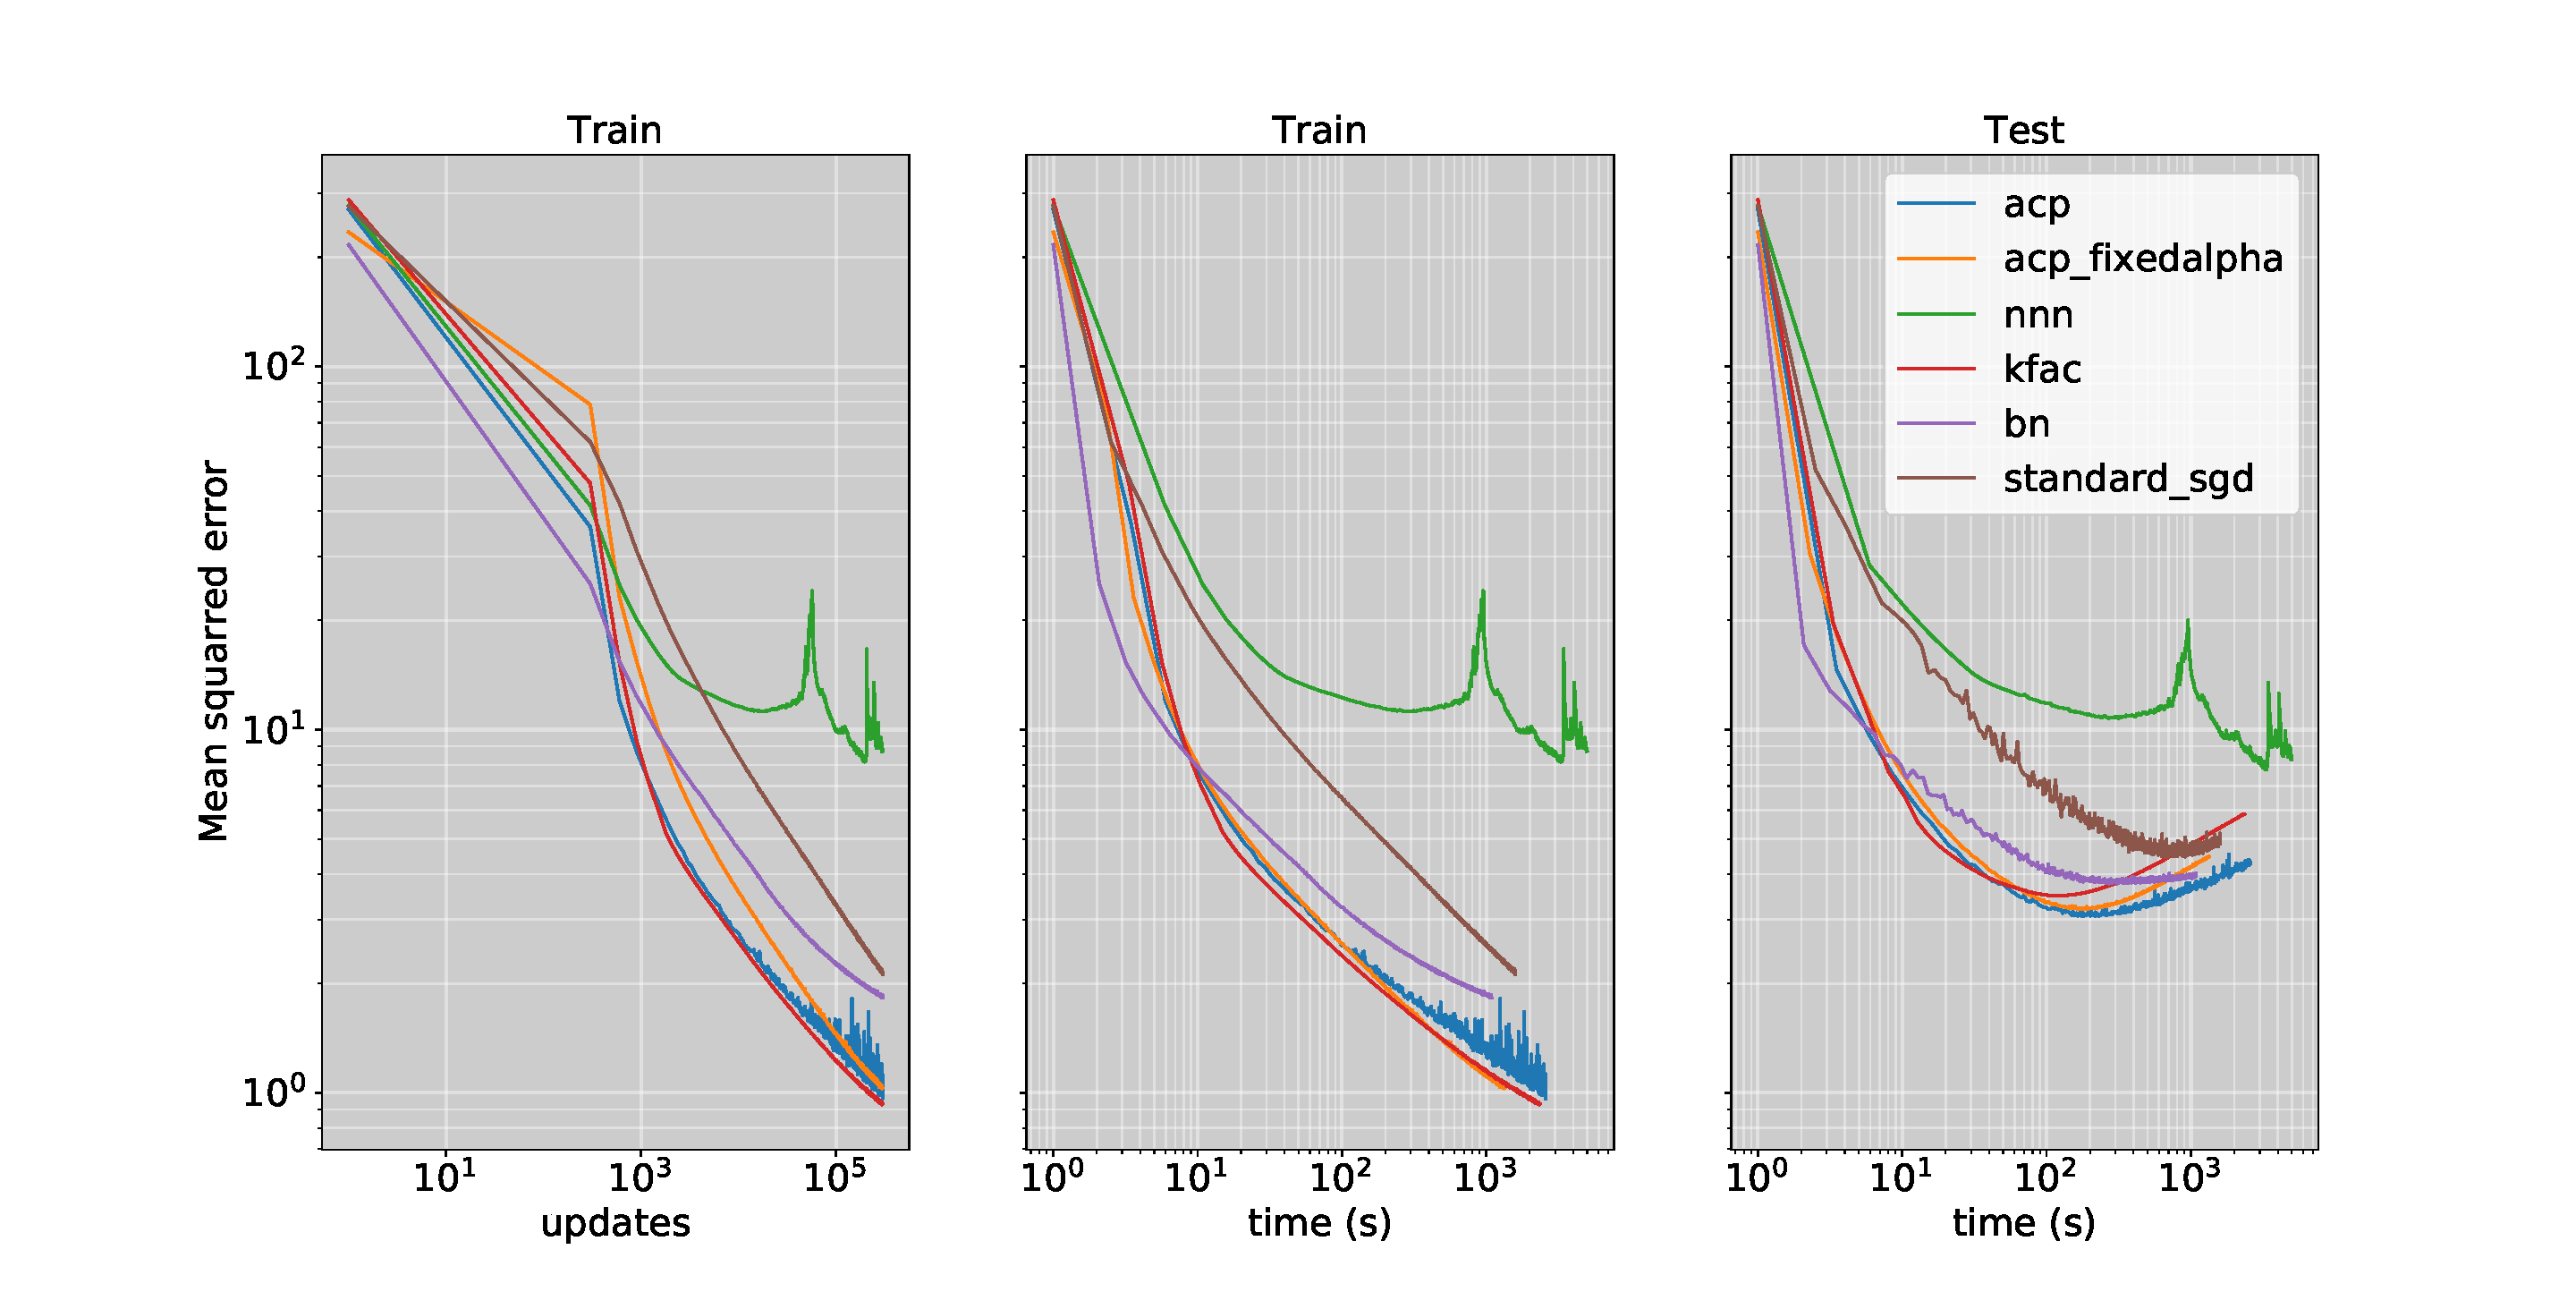
\includegraphics[width=1\textwidth]{figures/2nd}

\caption{Comparison of second order methods on MNIST autoencoder: blue: ACP
with fixed $\alpha$ as presented in section \ref{subsec:Amortized-covariance-preconditio};
orange: ACP with heuristic for $\alpha$ as presented in section \ref{subsec:Amortized-covariance-preconditio};
green: Natural Neural Network; red: KFAC; purple: batch norm with
standard SGD; brown: standard SGD}
\label{mnist-autoencoder}
\end{figure}

\begin{figure}[h]
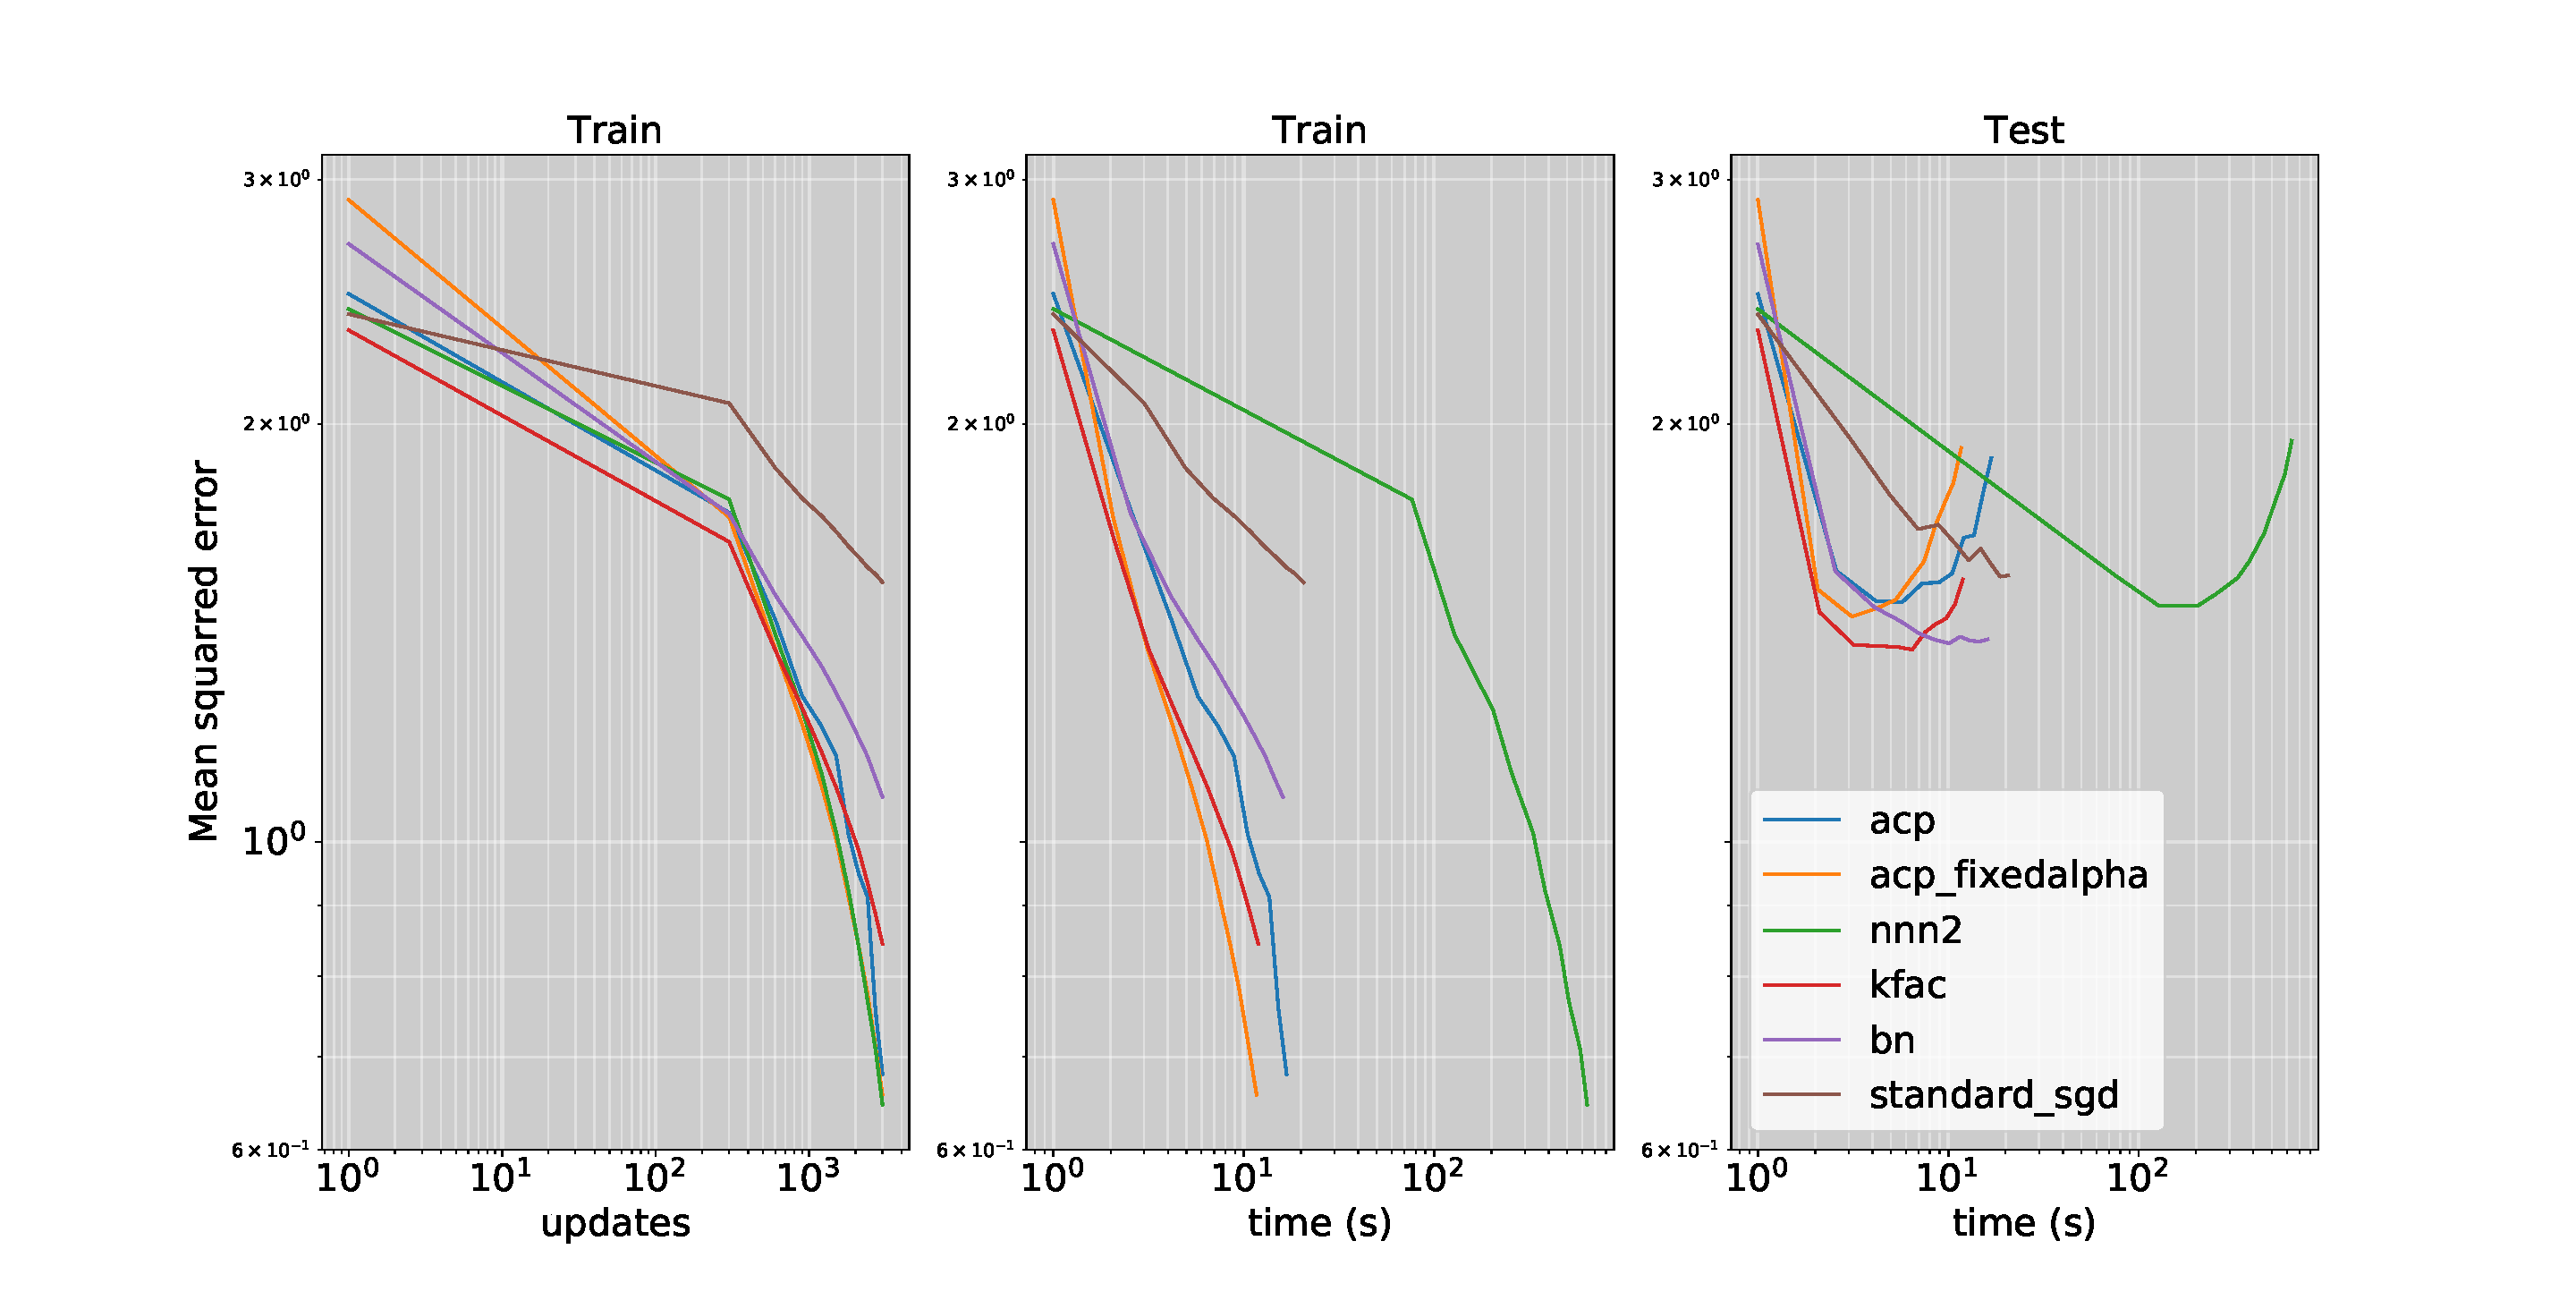
\includegraphics[width=1\textwidth]{figures/cifar10}

\caption{Comparison of second order methods on CIFAR10 classification: blue:
ACP with fixed $\alpha$ as presented in section \ref{subsec:Amortized-covariance-preconditio};
orange: ACP with heuristic for $\alpha$ as presented in section \ref{subsec:Amortized-covariance-preconditio};
green: Natural Neural Network; red: KFAC for Gauss-Newton; purple:
batch norm with standard SGD; brown: standard SGD; pink: KFAC for
natural gradient}
\label{cifar10}
\end{figure}


\subsection{Interpretation and conclusions}

\subsubsection{How do all second order methods compare ?}

In terms of updates, our best performer is the natural gradient approximated
by KFAC on both experiments. But in the case of the autoencoder, we
see that because it is faster to compute only the forward statistics,
ACP and KFAC compare similarly. Note that for the autoencoder, the
best test set is attained by ACP, and also in a shorter time than
all other methods.

\subsubsection{Does the improvement come from the centering trick or from the covariances
?}

In the centering experiment, we clearly see that full ACP outperforms
all centered activation methods by a large margin. Centered gradient
descent does not even improve on SGD. This is in contradiction with
our early experiments on a smaller number of iterations, which showed
much better progress for early training. The best performing centered
gradient is mean only batch norm. In addition to centering the gradients,
it also probably better condition the problem by modifying the backpropagated
gradients.

We can thus conclude that the improvement of ACP and other second
order methods does not only come from centering the activations, but
also from the full covariance.

\subsubsection{Stability}

There is a stability issue with ACP visible on the blue curve in figure
\ref{cifar10}. Recall that we divide the Tikhonov regularization
factor by a varying $\alpha$, proportional to the gradient incoming
in the current layer. This stability issue could probably be eased
with regularization by adding a small scalar value before dividing.

\subsubsection{How does KFAC compare to KFAC for Gauss-Newton ?}

As mentionned, the FIM and the GN are the same for the quadratic error.
But this is not the case for the cross entropy. Both methods can be
decomposed using the Kronecker product of 2 small matrices, so we
want to compare how they perform. As can be seen in figure \ref{cifar10}
by comparing the red curve for GN and the pink curve for FIM, we observe
that the natural gradient version performs much better than the GN
version, with respect to both the number of updates and the wallclock
time. It is remarkable as the natural gradient version takes much
longer to recompute stats, because it needs the whole jacobians of
the output of the network, whereas GN only needs the gradient, so
there is no additional cost for the backpropagation as we mentionned
in section \ref{sec:gn-trick-cheap}.

\chapter*{Conclusions}

During this work, we derived new expressions for the well known GN
matrix and FIM. We showed that there is a common factor in both matrices
that is composed of the covariance matrix of the activation at each
layer, in the case of a block diagonal approximation. By separating
the bias and the weight matrices we introduced a new mathematical
explanation for the well-known centering trick. Using this new expressions
we derived a new algorithm ACP that loosely resembles 2 state of the
art methods inspired by natural gradient. We benchmarked our new algorithm
against these methods and showed that they all perform similarly.

We also introduced a tentative modification of backpropagation in
order to obtain better derivatives. This algorithm showed promising
result since it provided better updates than vanilla gradient descent.
However there remains some limits to applying this technique in a
real setup as it is still too computationnally expensive.

A natural follow-up to this work is to extend it to other architectures
such as recurrent neural networks as formally initiated in \citet{ollivier2015riemannian}
or convolutional networks such as in \citet{grosse2016kronecker}.
Networks with very small outputs can also be good candidates as computing
the jacobians thus the FIM is linear in the number of outputs. Amongst
them is the very popular family of GAN networks where the output is
a single unit, and where the natural gradient could be used as a way
to stabilize the training by balancing the rate of change of the output
from each part (generator and discriminator).

Another direction of pursuing this research is to look for better
approximations of the layer FIM/GN than the one of splitting into
2 expectations. Indeed, by better we do not mean an approximation
that is closer in norm to the real FIM, but instead to an approximation
that will give updates that are more efficient. Amortization can also
be improved, by monitoring how our inverse statistics stay close to
the true statistics, and just performing updates of these preconditioner
when it is necessary, allowing for less updates (and less matrix inversions)
for layers where the statistics do not change much.

As a last word, let us just state that second order methods have proven
very powerful in a wide variety of optimization problems, but suffer
from their computation complexity and the difficulty to use them in
a setup with a lot of variables to optimize. We hope that by pursuing
this effort of clarifying things and finding approximate methods that
are computationnally cheaper, we will carry on contributing to more
efficient neural network training.


\end{document}
